%!TEX root = ../report.tex

\begin{document}
	\let\cleardoublepage\clearpage
    \section{Analyzing existing sensor data model specifications}
    In this section, we analyze the existing data model specifications which are widely used to represent sensor generated data. Additionally, to find out best context based data models we reviewed Resource Description Framework and JSON-LD.
    
    \subsection{SenML}
    SenML is an encoding format to represent the sensor values as simple as possible; therefore a simple microcontroller can process it with little memory and computation resource.
    
    Single SenML message can consist of an array of sensor measurements along with minimal additional information to describe the sensor itself. This information will solve the interoperability when other systems try to understand the data. However, due to efficiency reasons, it can hold only a few meta information such as sensor name, and their unit. Before analyzing the examples, we can look at the semantics defined by SenML in the below table \ref{tab:senml_semantics}.
    
    
    \begin{table}[h!]
    		\begin{tabular}{|l|p{12cm}|} % <-- Alignments: 1st column left, 2nd middle and 3rd right, with vertical lines in between
    			\hline
    			\textbf{Semantics} & \textbf{Definitions}\\
    			\hline
    			
    			bn & Base name which is used to attach before all the names in the measurement and it will reduce the size of the complete message. \\
    			\hline
    			bt & Base time represents the start time of the first measurement being measured.\\
    			\hline
    			bu &	Base unit, it will be useful if all the measurements have the same unit.\\
    			\hline
    			bv &	Base value, it will be added to the values in the measurement.\\
    			\hline
    			bver &	Version of the SenML media format.\\
    			\hline
    			n &	Name of a sensor, and base name will be prepended with this name.\\
    			\hline
    			u &	Represents the units of the observed measurement.\\
				\hline
    			v &	The value (number) generated by the sensor.\\
    			\hline
    			vs &	String value.\\
    			\hline
    			vb &	Boolean value.\\
    			\hline
    			vd &	Data value (base64 encoded string).\\
    			\hline
    			s &	Value sum.\\
    			\hline
    			ut &	Update time.\\
    			\hline
    			t &	Time.\\
    			\hline
    		\end{tabular}
    	    \caption{SenML semantics used to build SenML messages}
	    	\label{tab:senml_semantics}
    \end{table}
    
%    The figure shows the possible basic example of SenML structure to represent a sensor generated data, and the data holds a single observation of voltage from a voltage sensor.
     Figure \ref{fig:senml_simple} shows the possible basic example of SenML structure to represent a sensor generated data, and the data holds a single observation of voltage from a voltage sensor.
    
    \begin{figure}[!htbp] 
    	\begin{center}
    		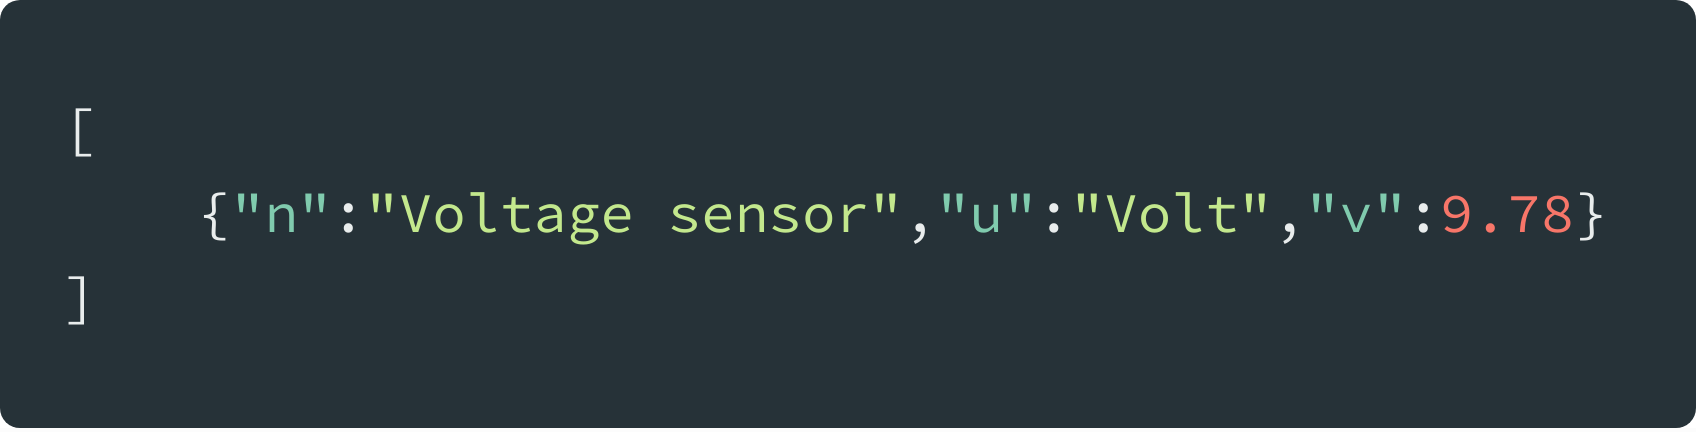
\includegraphics[scale=0.1]{./images/png/senml/simple}	
    		\caption{Simple SenML observation structure}	
    		\label{fig:senml_simple}	
    	\end{center}
    \end{figure}

       
    
    
    Figure \ref{fig:senml_complex} shows a complex group of measurements which includes values from voltage and humidity sensors. While retrieving these measurements, the base name will be prepended with names and base unit 'RH' will also be added to all measurement except for those measurements that have a unit. For instance, in the above example voltage measurement have its unit 'V' attached to it already. So in this case, the base unit will not be added to this measurement.
    
    \begin{figure}[!htbp] 
    	\begin{center}
    		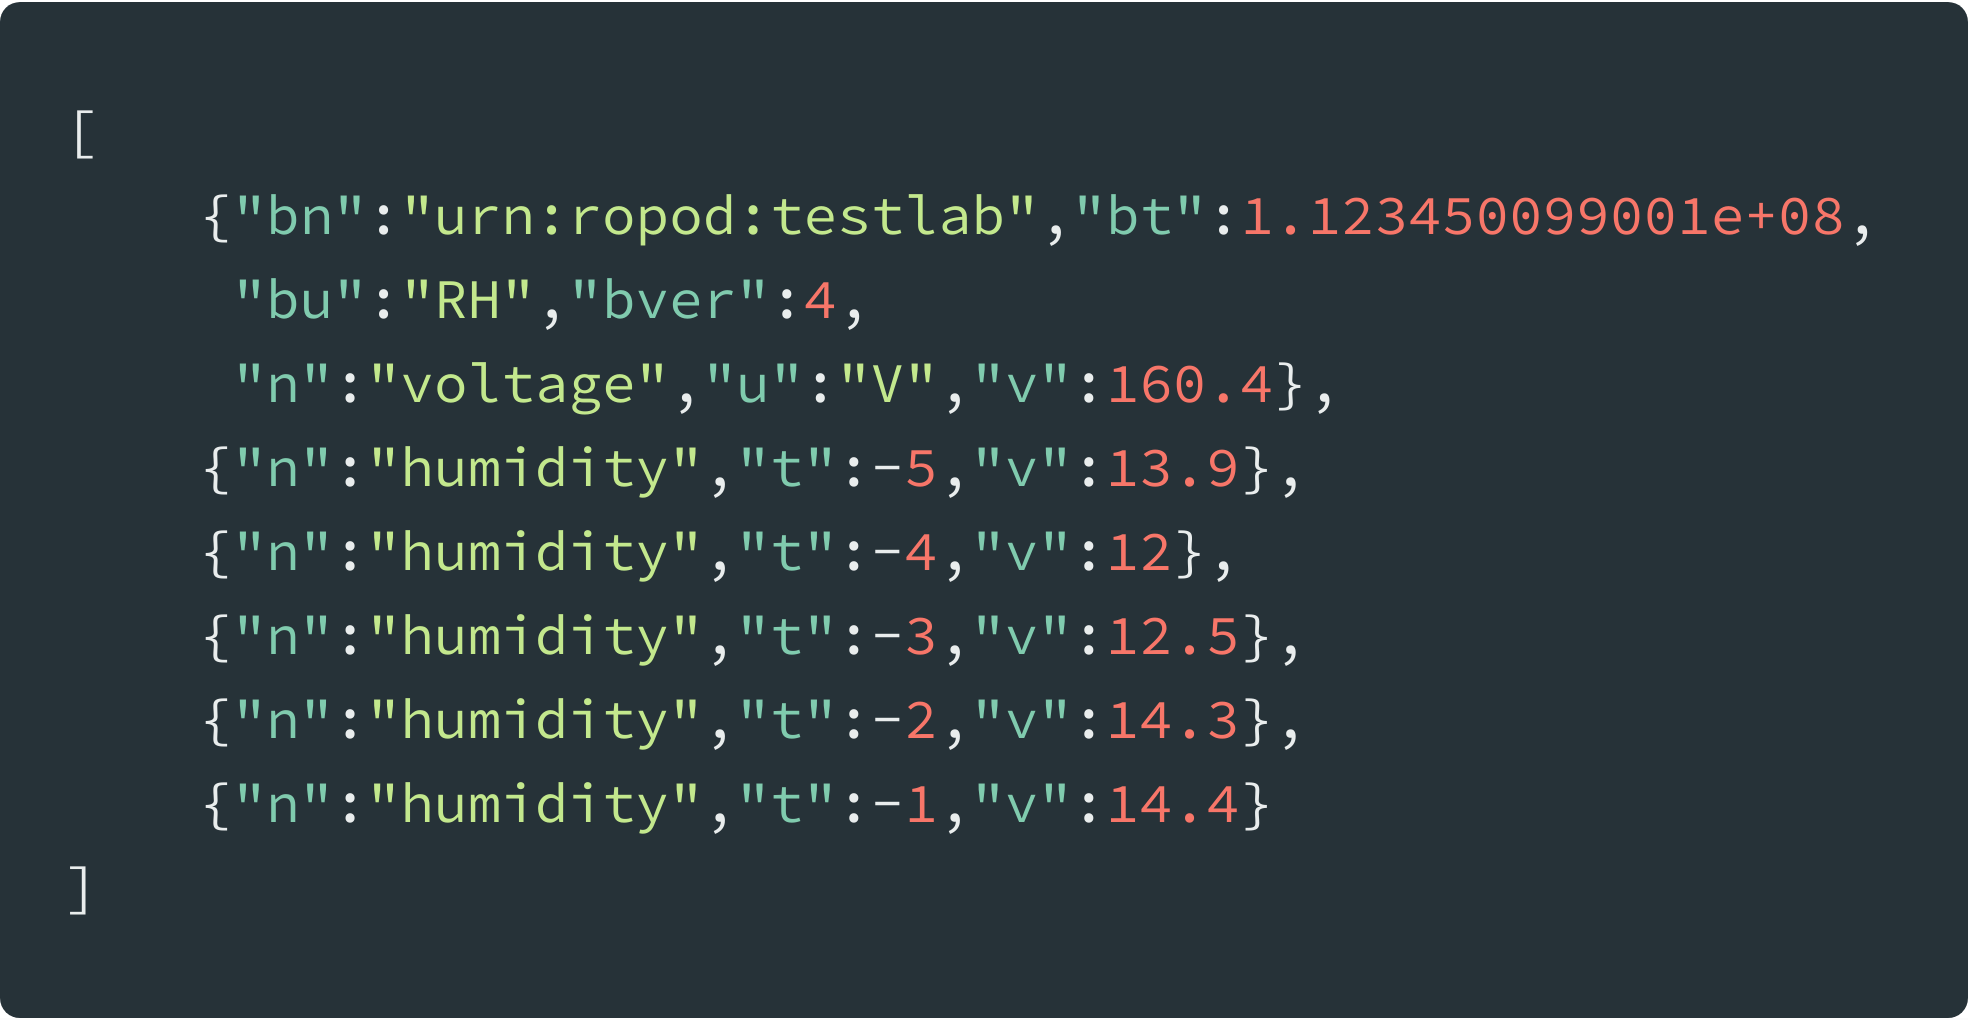
\includegraphics[clip,scale=0.14]{./images/png/senml/complex}	
    		\caption{Complex SenML observation structure}	
    		\label{fig:senml_complex}	
    	\end{center}
    \end{figure}

	To process or semantically query complex sensor data, measurements should have additional context about the data. However, it is not achievable directly with SenML, instead of as explained in this article \cite{su2014connecting} with the help of transformation from SenML to RDF one can explicitly specify the context of each measurement.
	
	\subsection{OGC SensorThings API}
	OGC SensorThings API offers a unique way to connect sensors in IoT platform and an entity based relationship model for handling data from heterogeneous sensors. It has two major components, one for sensing part and other for tasking part. For our research work, we are not going to review the Tasking part, since our focus is towards finding a better context-based data model for robotic applications.
	
	Sensing part follows the Observation and Measurement model from "OGC 10-004r3 and ISO 19156:2011". There are eight entities defined by SensorThings API.
	
	\subsubsection{Thing}
	Thing represents the physical things in the world or a virtual system that can be communicated via the network. Things have their own attributes such as name, description, and properties. A single thing can have many optional locations, historical locations, and data streams. The constraint is a thing that should be mapped to a single location at a given point of time.
	
	\begin{figure}[!htbp] 
		\begin{center}
			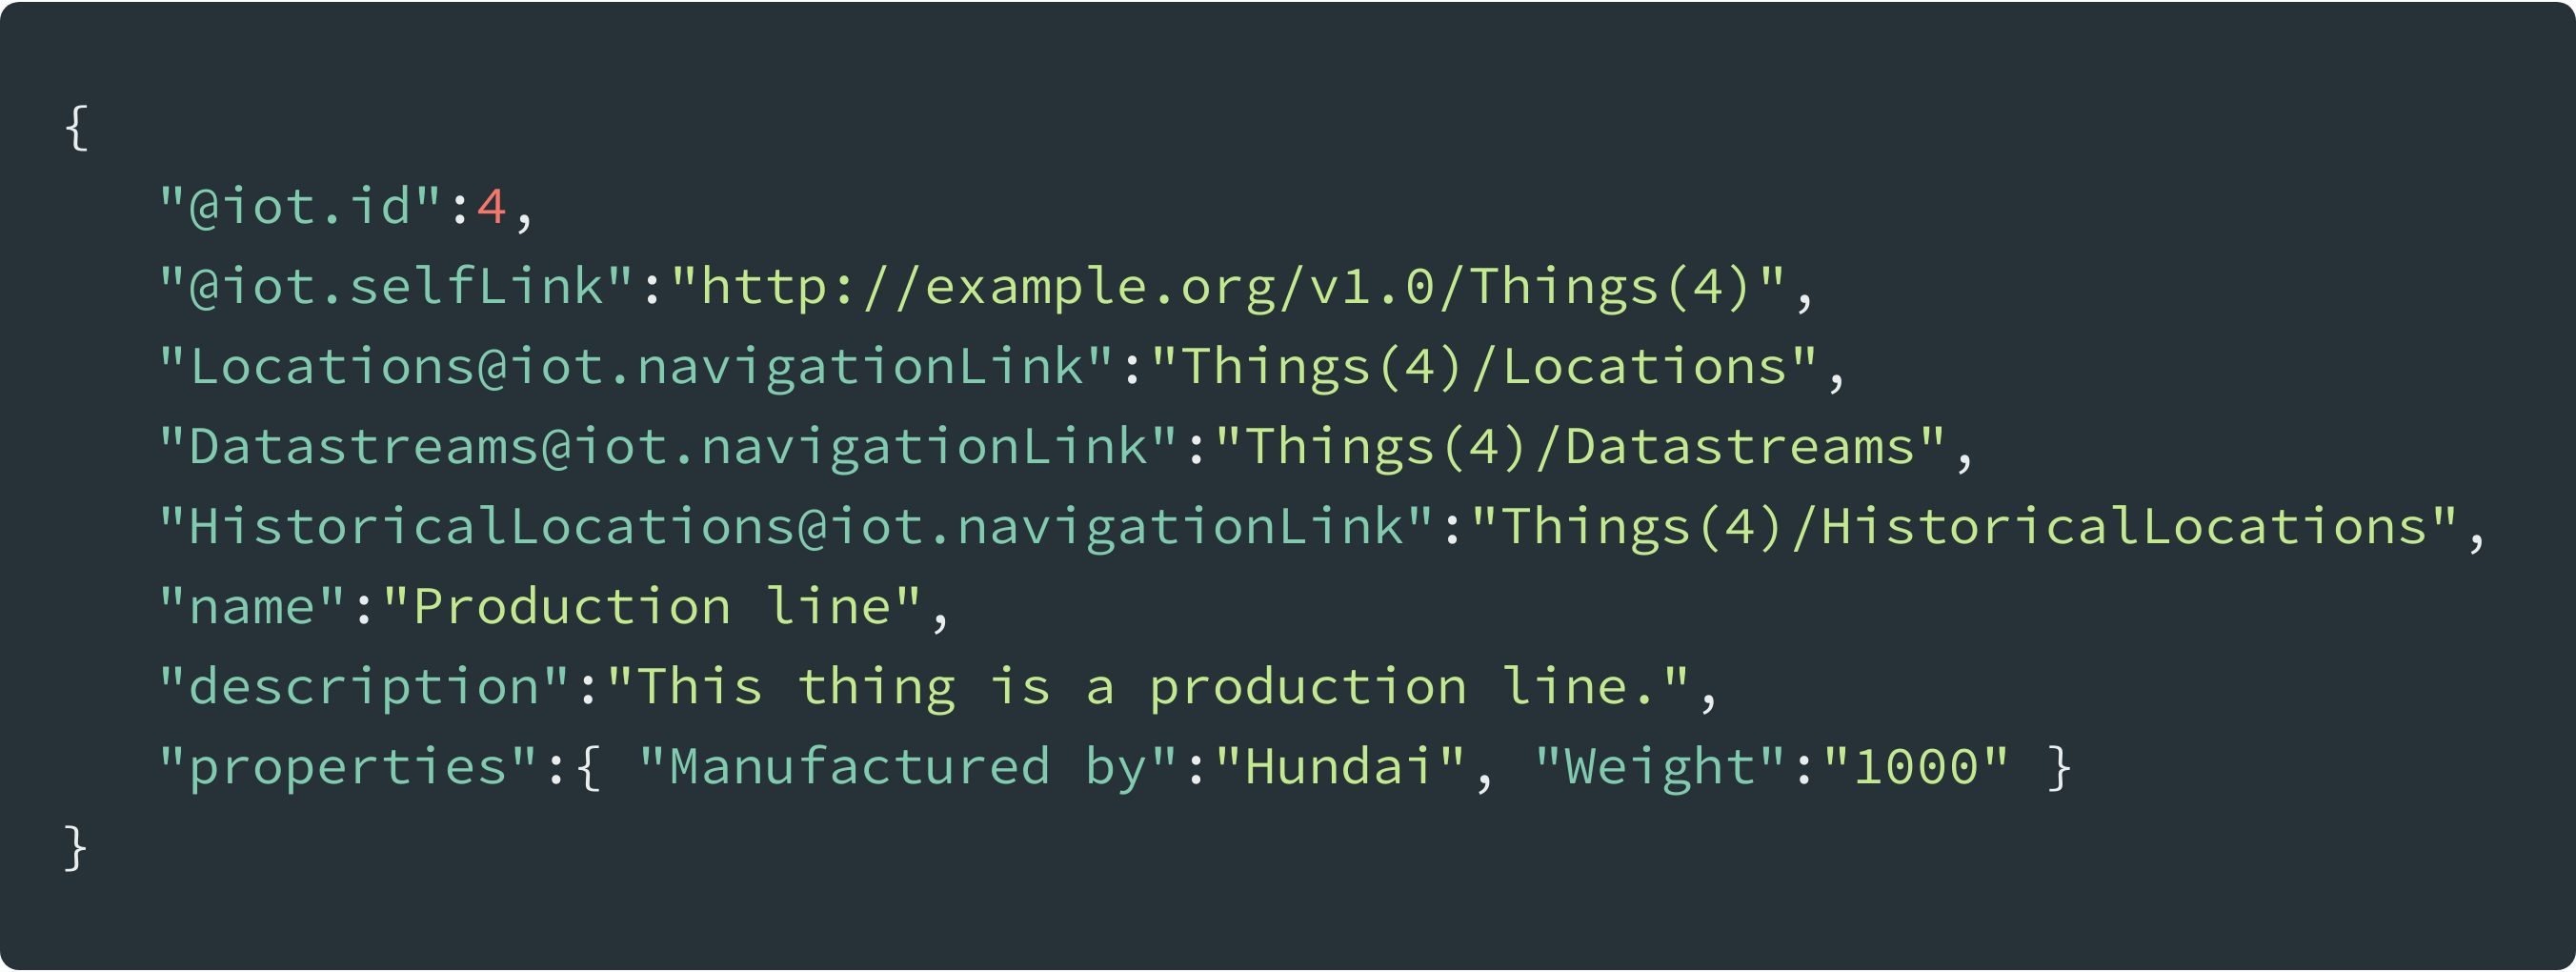
\includegraphics[scale=0.1]{./images/png/ogc/thing}	
			\caption{Structure of Thing entity}	
			\label{fig:thing}	
		\end{center}
	\end{figure}

	\subsubsection{Location}
	Location shows the coordinates of the real location and each location may locate multiple things. Each location should be provided with its encoding type to make the other robots/users quickly understand the location type and utilize them for calculation.
	
	\begin{figure}[!htbp] 
		\begin{center}
			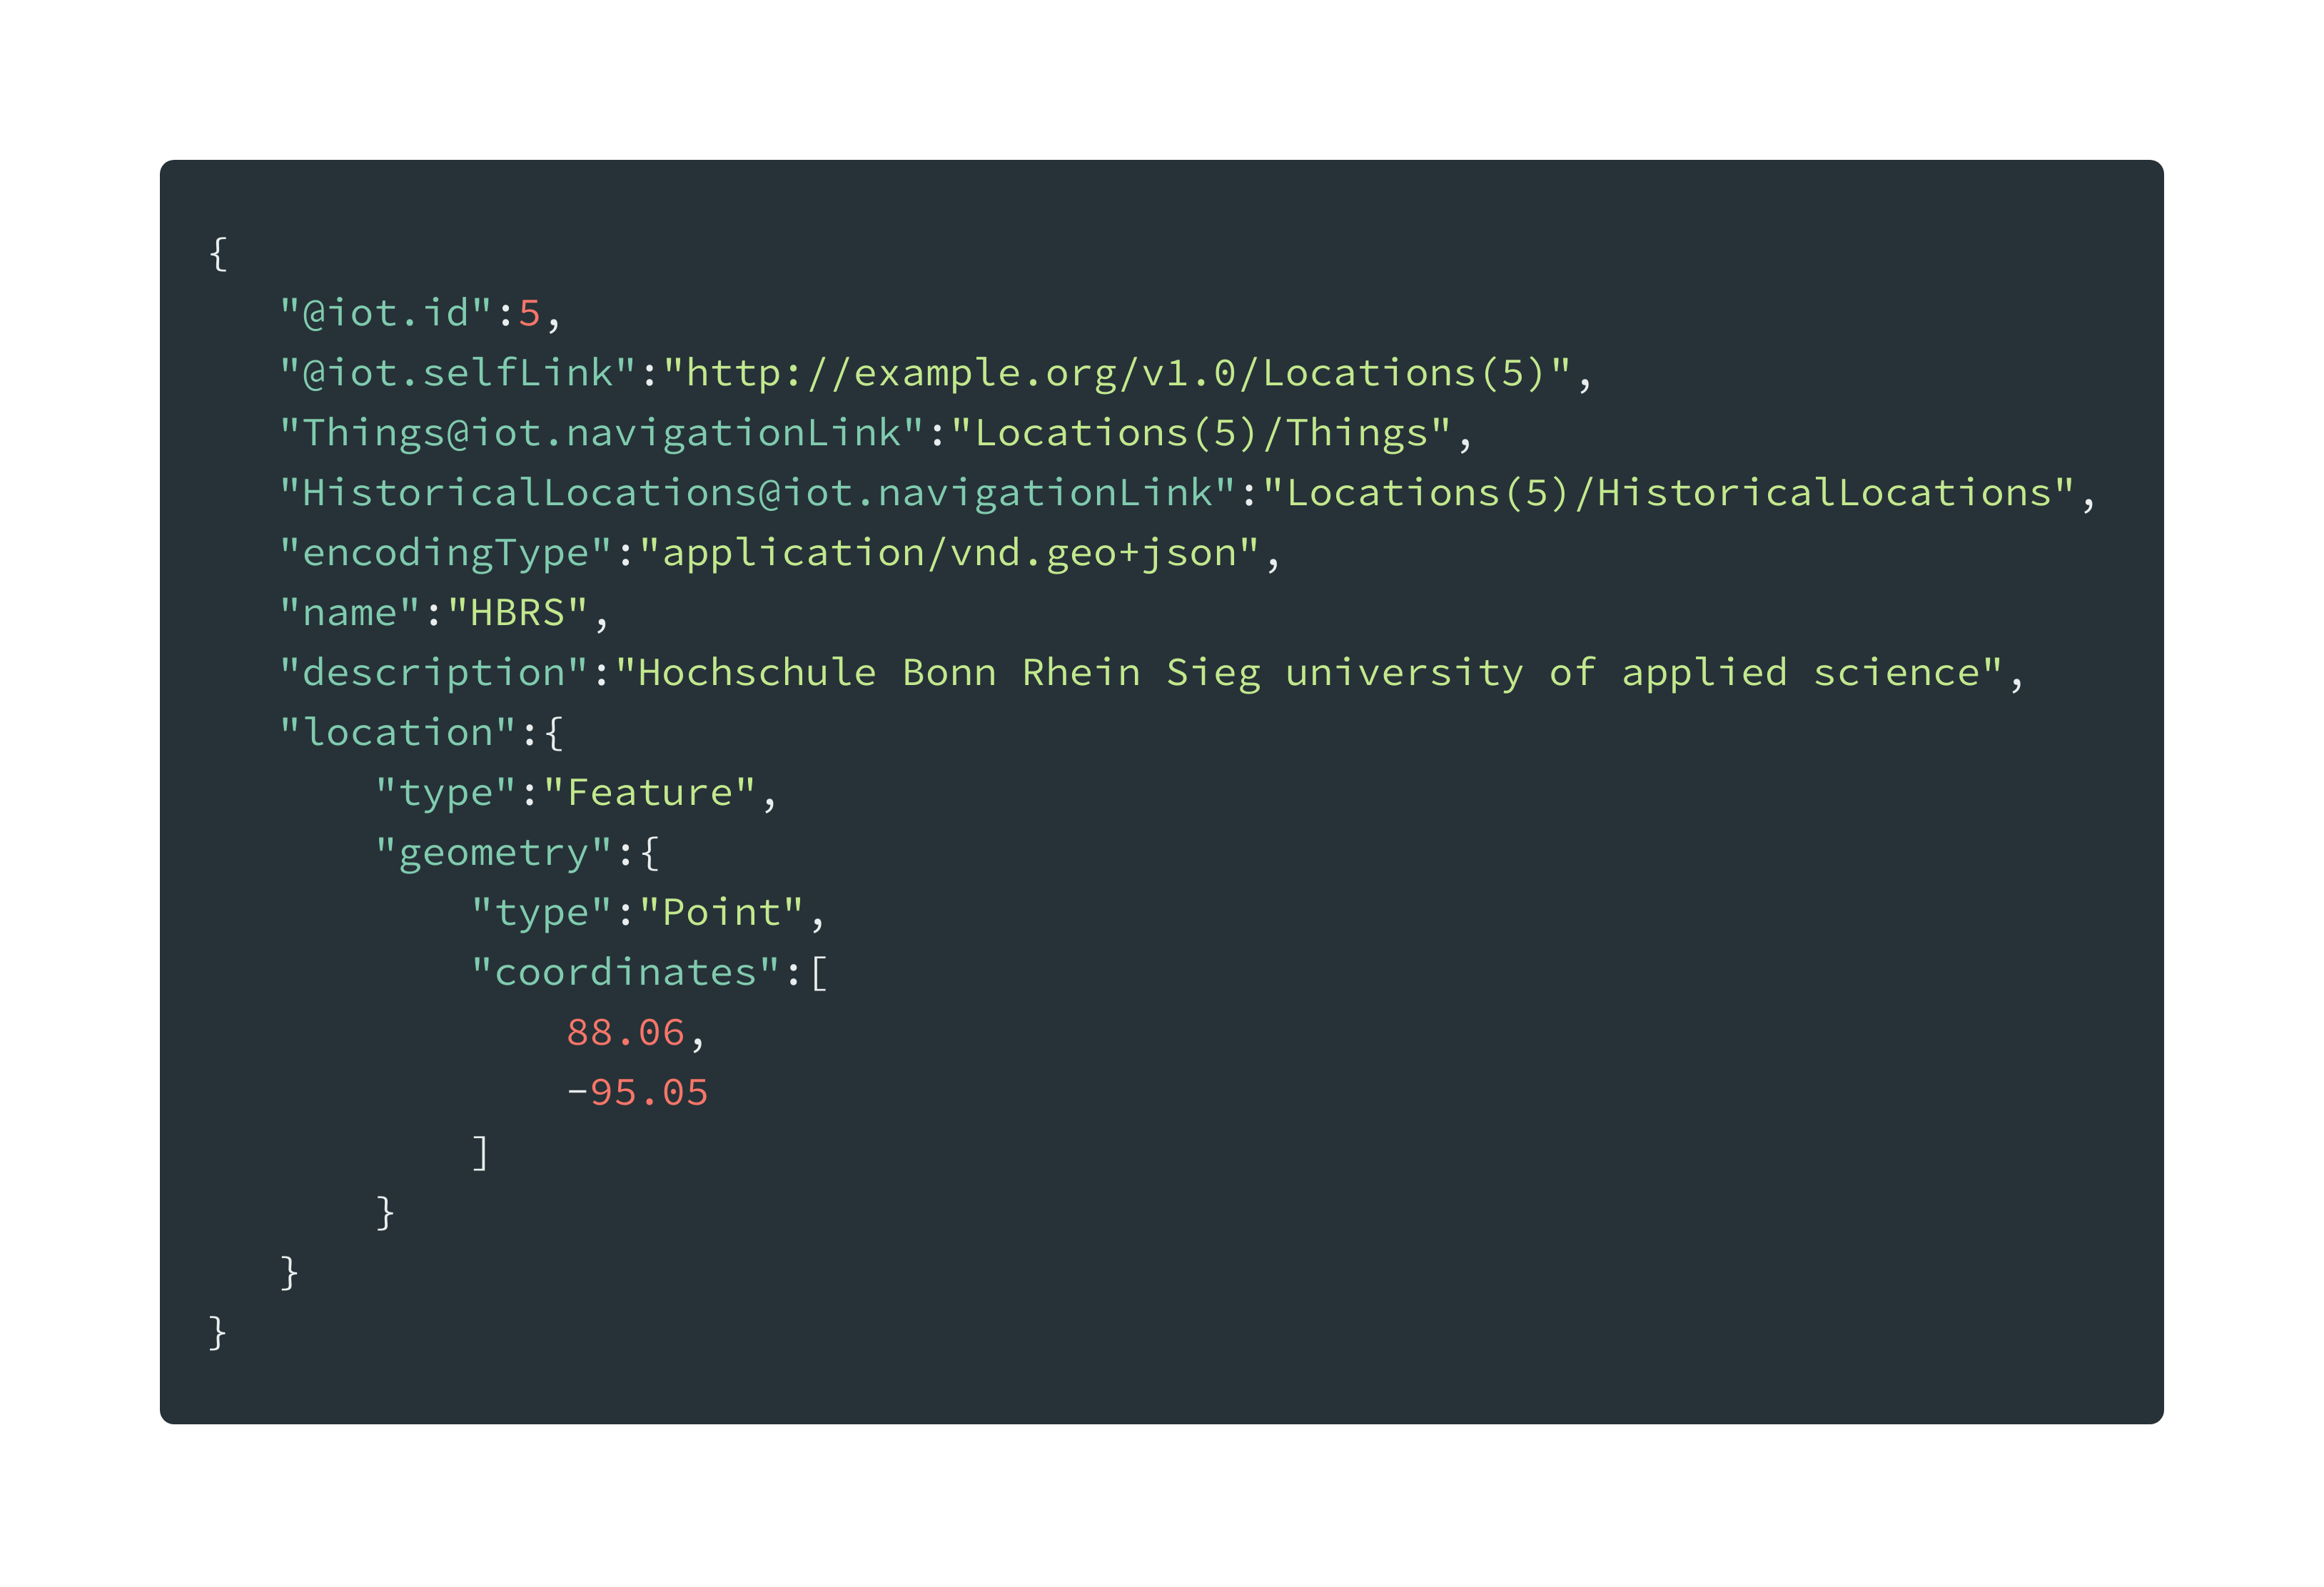
\includegraphics[scale=0.1]{./images/png/ogc/location}	
			\caption{Structure of Location entity}	
			\label{fig:location}	
		\end{center}
	\end{figure}

	\subsubsection{Sensor}
	Sensor entity represents the physical sensing device which generates the values. Each sensor should have at least one data stream entity relation. Each sensor is described along with its encodingTypa and an optional metadata field.
	
	\begin{figure}[!htbp] 
		\begin{center}
			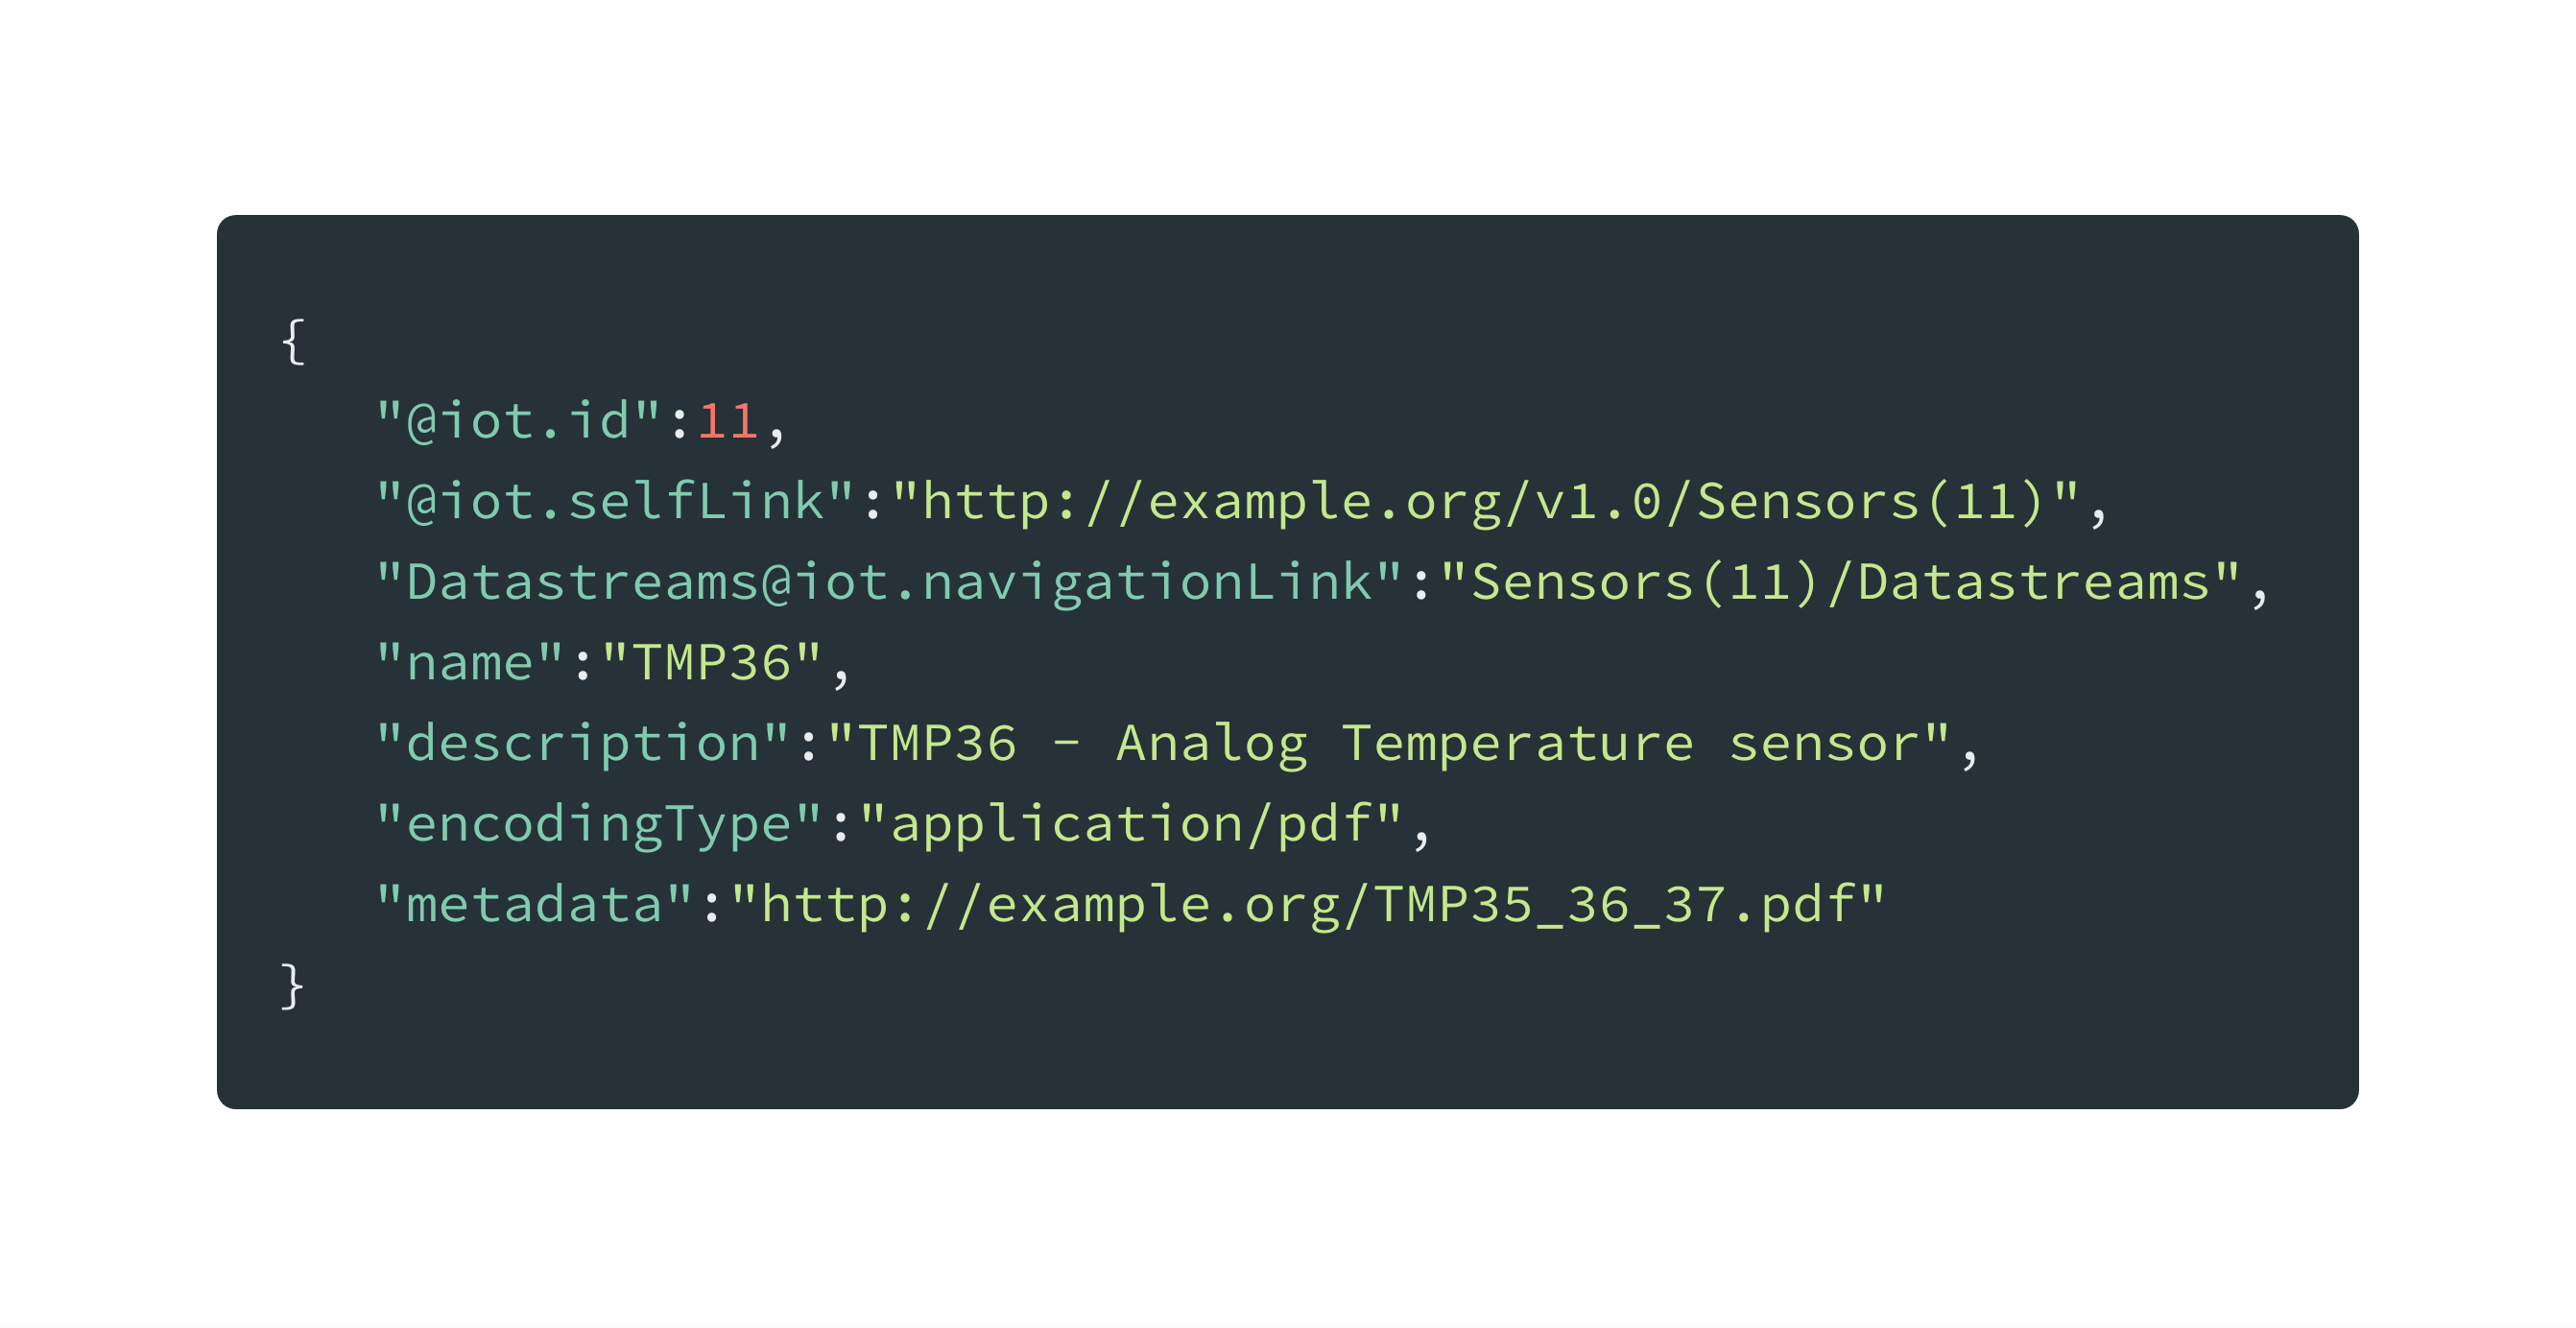
\includegraphics[scale=0.1]{./images/png/ogc/sensor}	
			\caption{Structure of Sensor entity}	
			\label{fig:sensor}	
		\end{center}
	\end{figure}

	\subsubsection{HistoricalLocation}
	HistoricalLocation shows the thing to be in the location or vice versa, at a given timestamp. For example, consider a robot (thing) is running from one room to another room for a specific task. To make the relation between the robot (thing) and the room (location), we create HistoricalLocation data with the reference of the robot and the room along with a timestamp. Timestamp plays a significant role here because it shows the truthness of the thing to be present physically in any given location.
	
	\begin{figure}[!htbp] 
		\begin{center}
			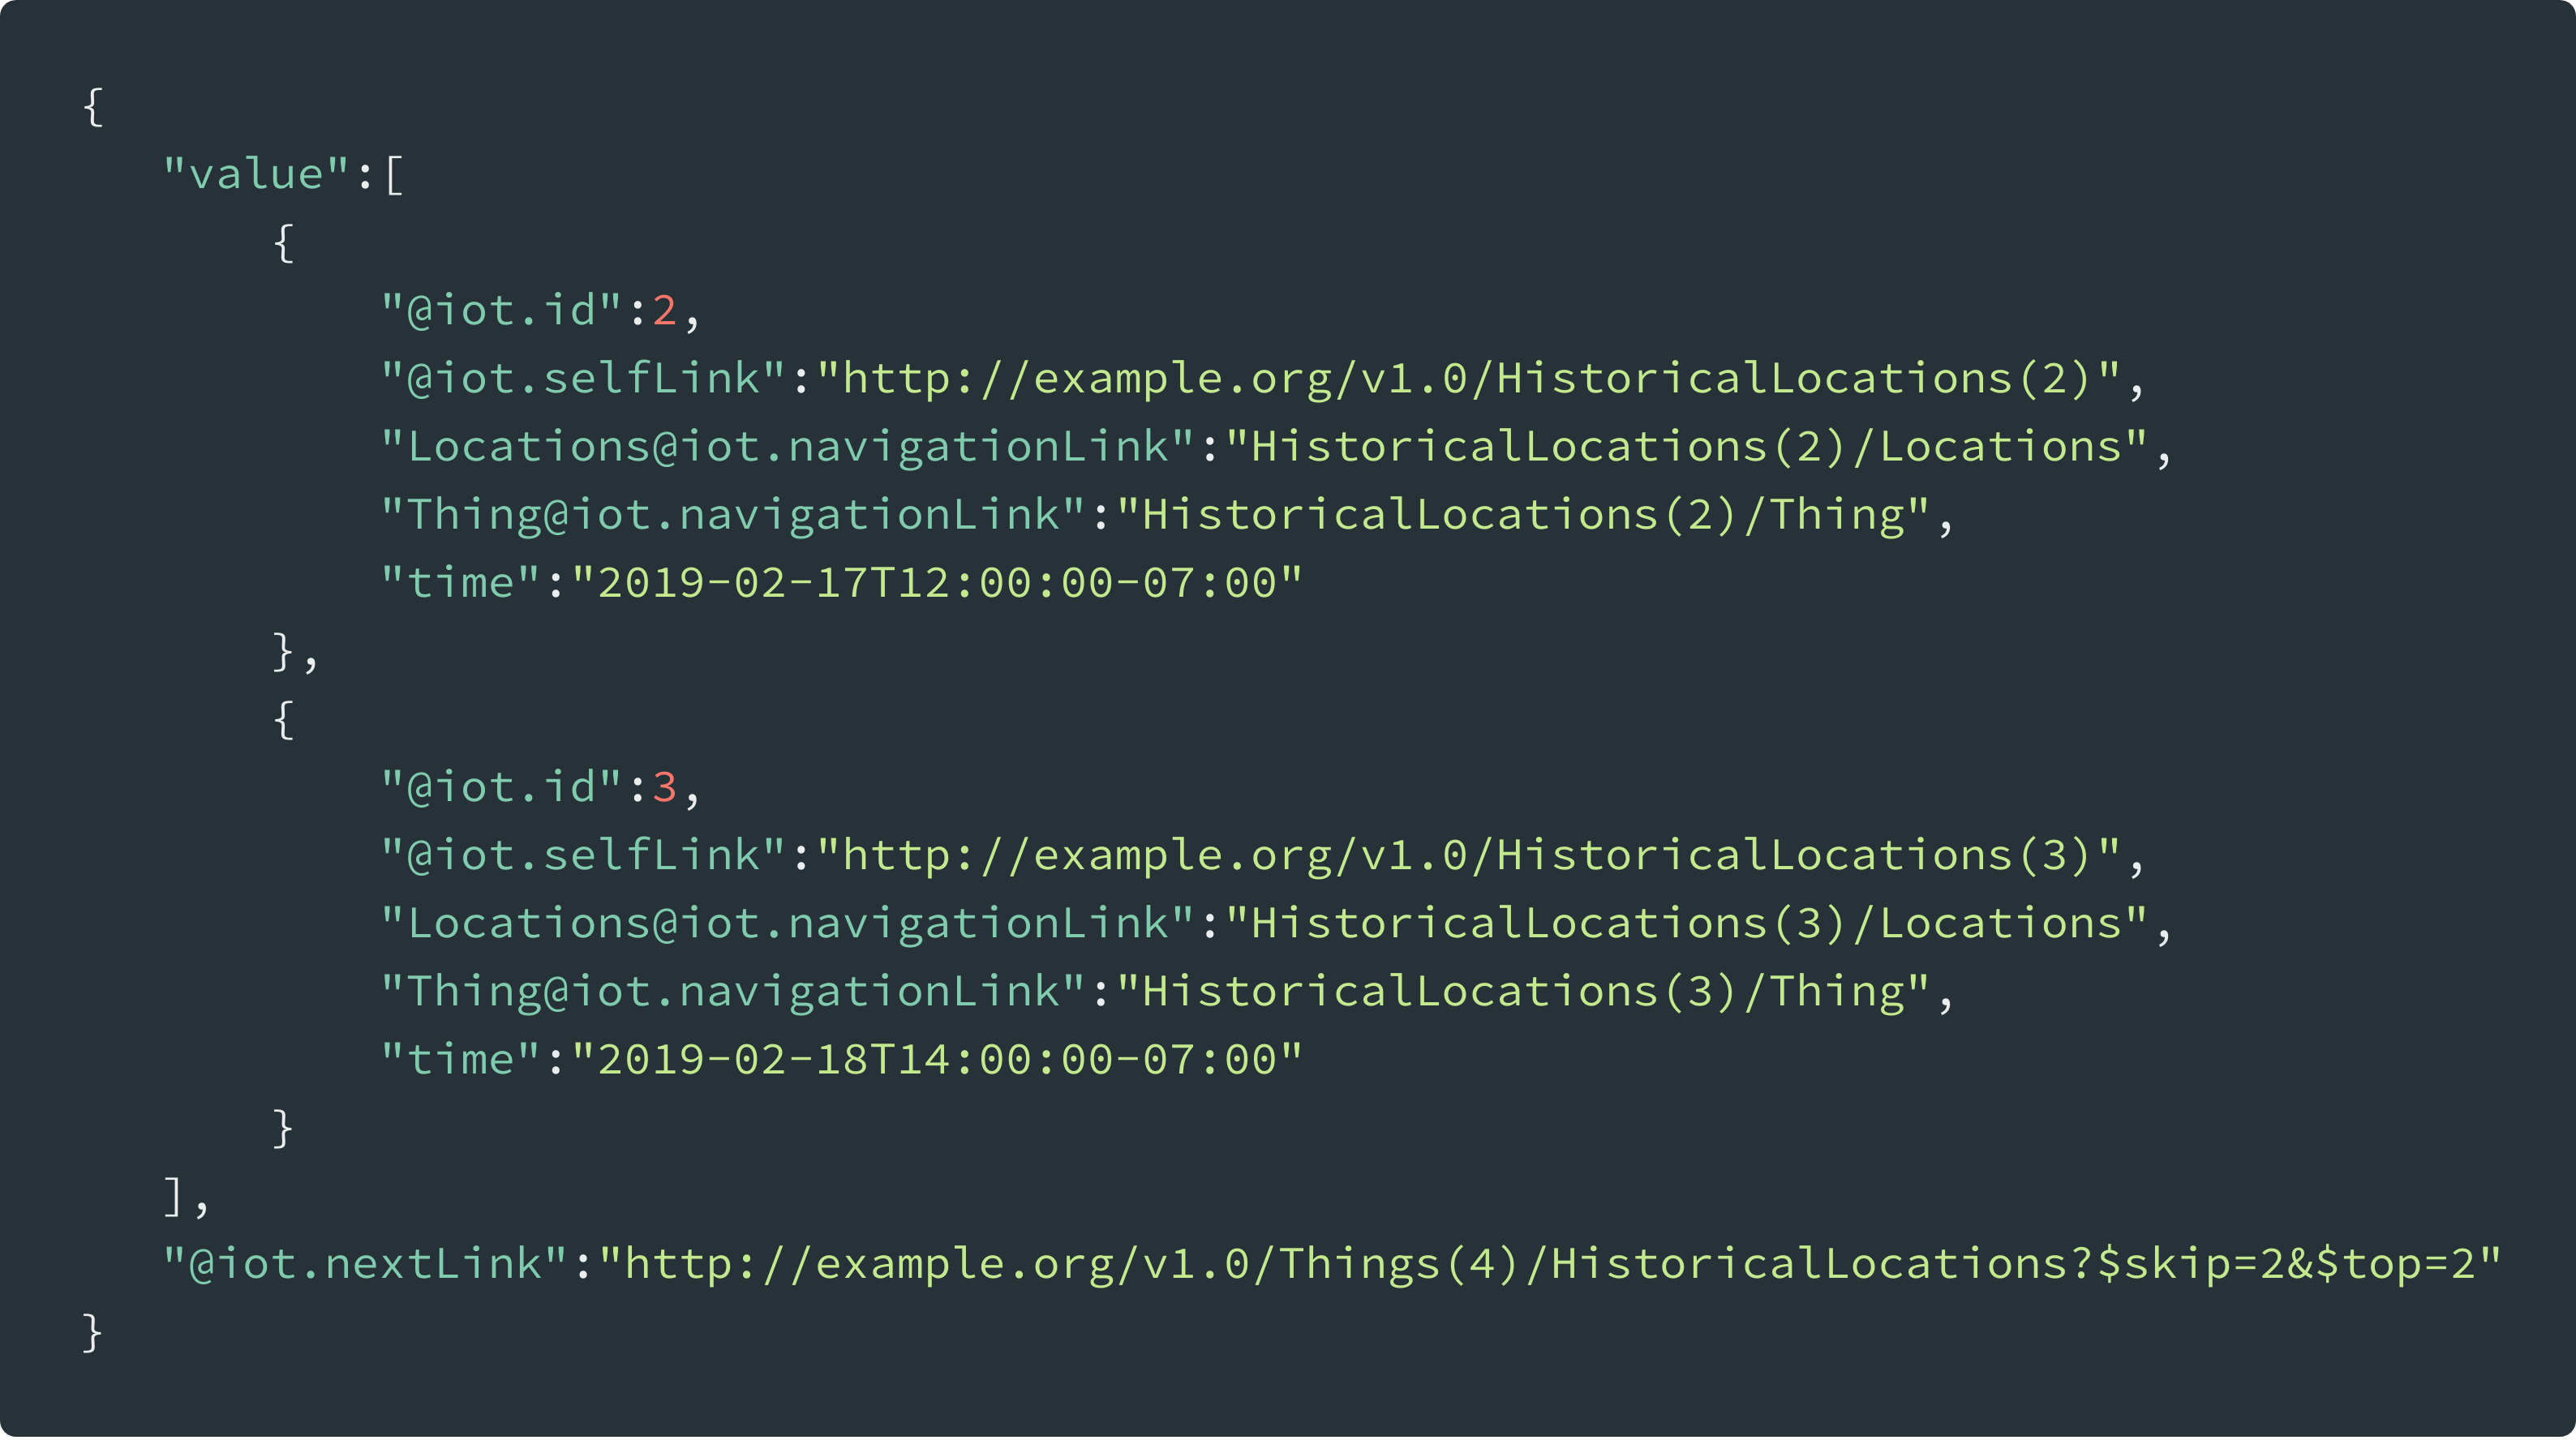
\includegraphics[scale=0.1]{./images/png/ogc/historical_location}	
			\caption{Structure of HistoricalLocation entity}	
			\label{fig:historical_location}	
		\end{center}
	\end{figure}



	\subsubsection{FeatureOfInterest}
	Each observation value represents the property of a feature, and with the help of FeatureOfInterest entity one can filter the observations easily. For example, FeatureOfInterest of a GPS sensor is location since it generates the coordinates of its current location.
	
	\begin{figure}[!htbp] 
		\begin{center}
			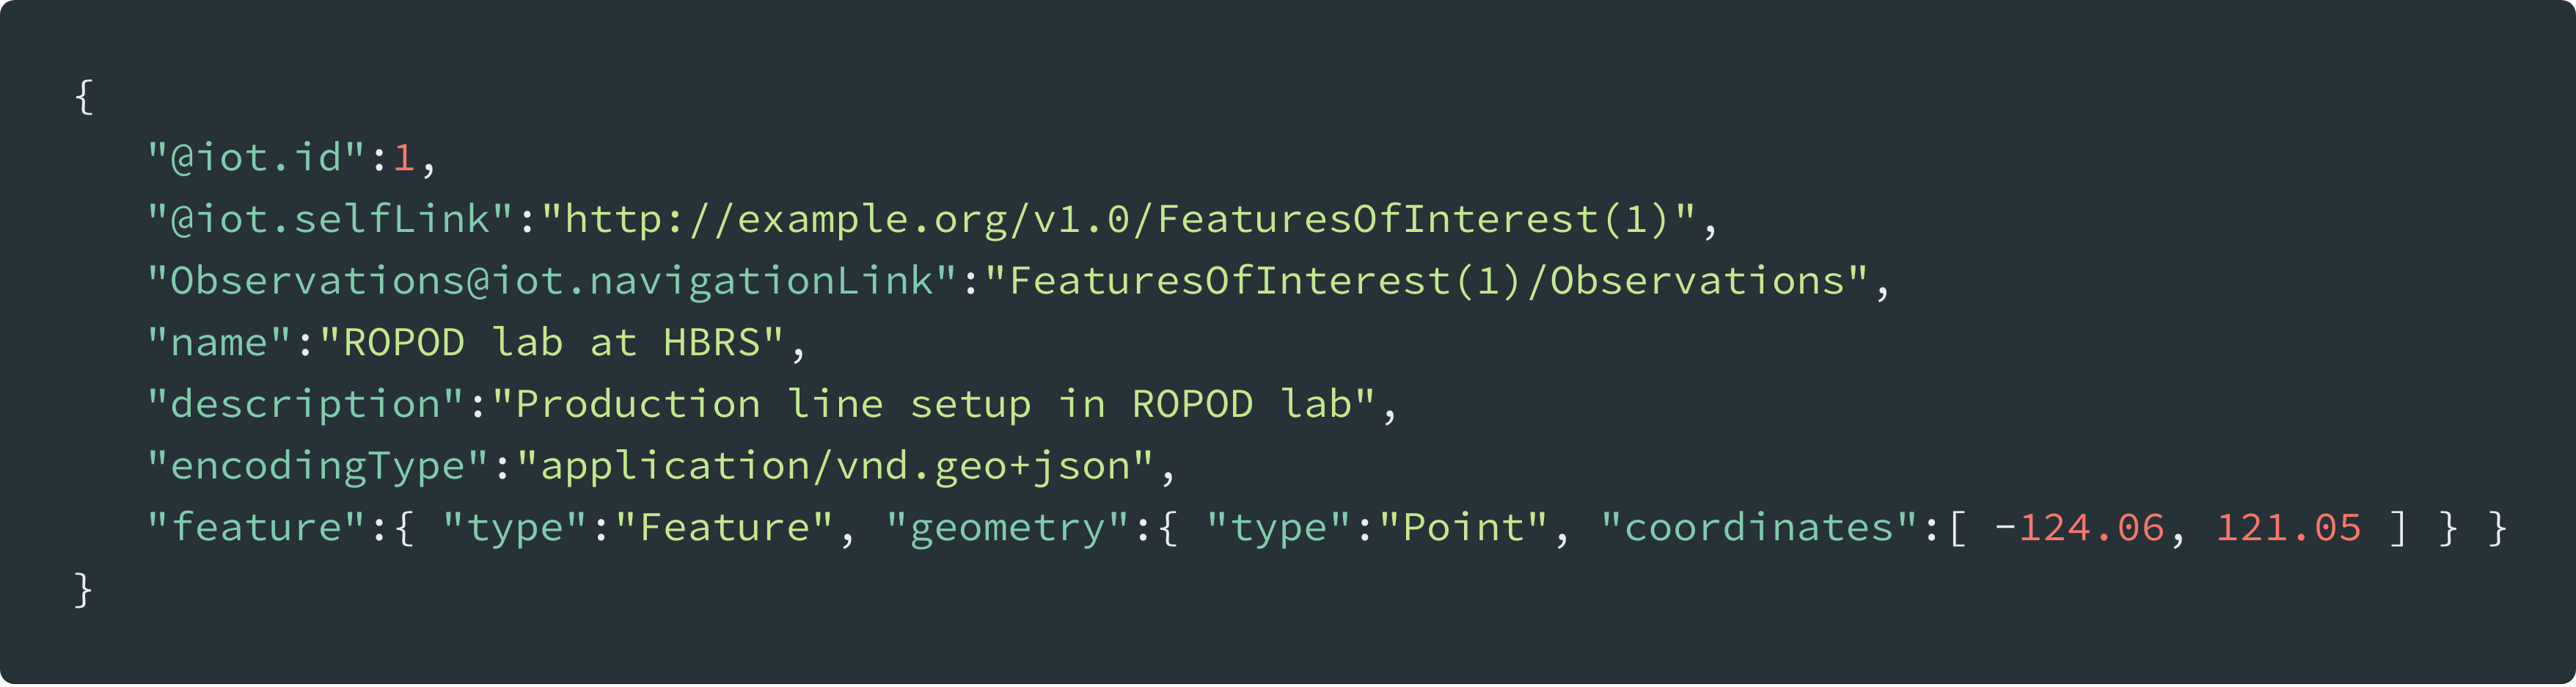
\includegraphics[scale=0.1]{./images/png/ogc/featureofinterest}	
			\caption{Structure of FeatureOfInterest entity}	
			\label{fig:featureofinterest}	
		\end{center}
	\end{figure}
	
	\subsubsection{Datastream}
	 Datastream stores the list of observations for a specific thing and a sensor. Each data stream should have at least one sensor and thing entity relationship. For example, a gateway (Thing) with a temperature sensor (Sensor) generates a list of temperature observations under Temperature Datastream.  Also, datastream holds the type of observation and area which defines the coordinates of the location from where the robot generates the actual observation.
	
	\begin{figure}[!htbp] 
		\begin{center}
			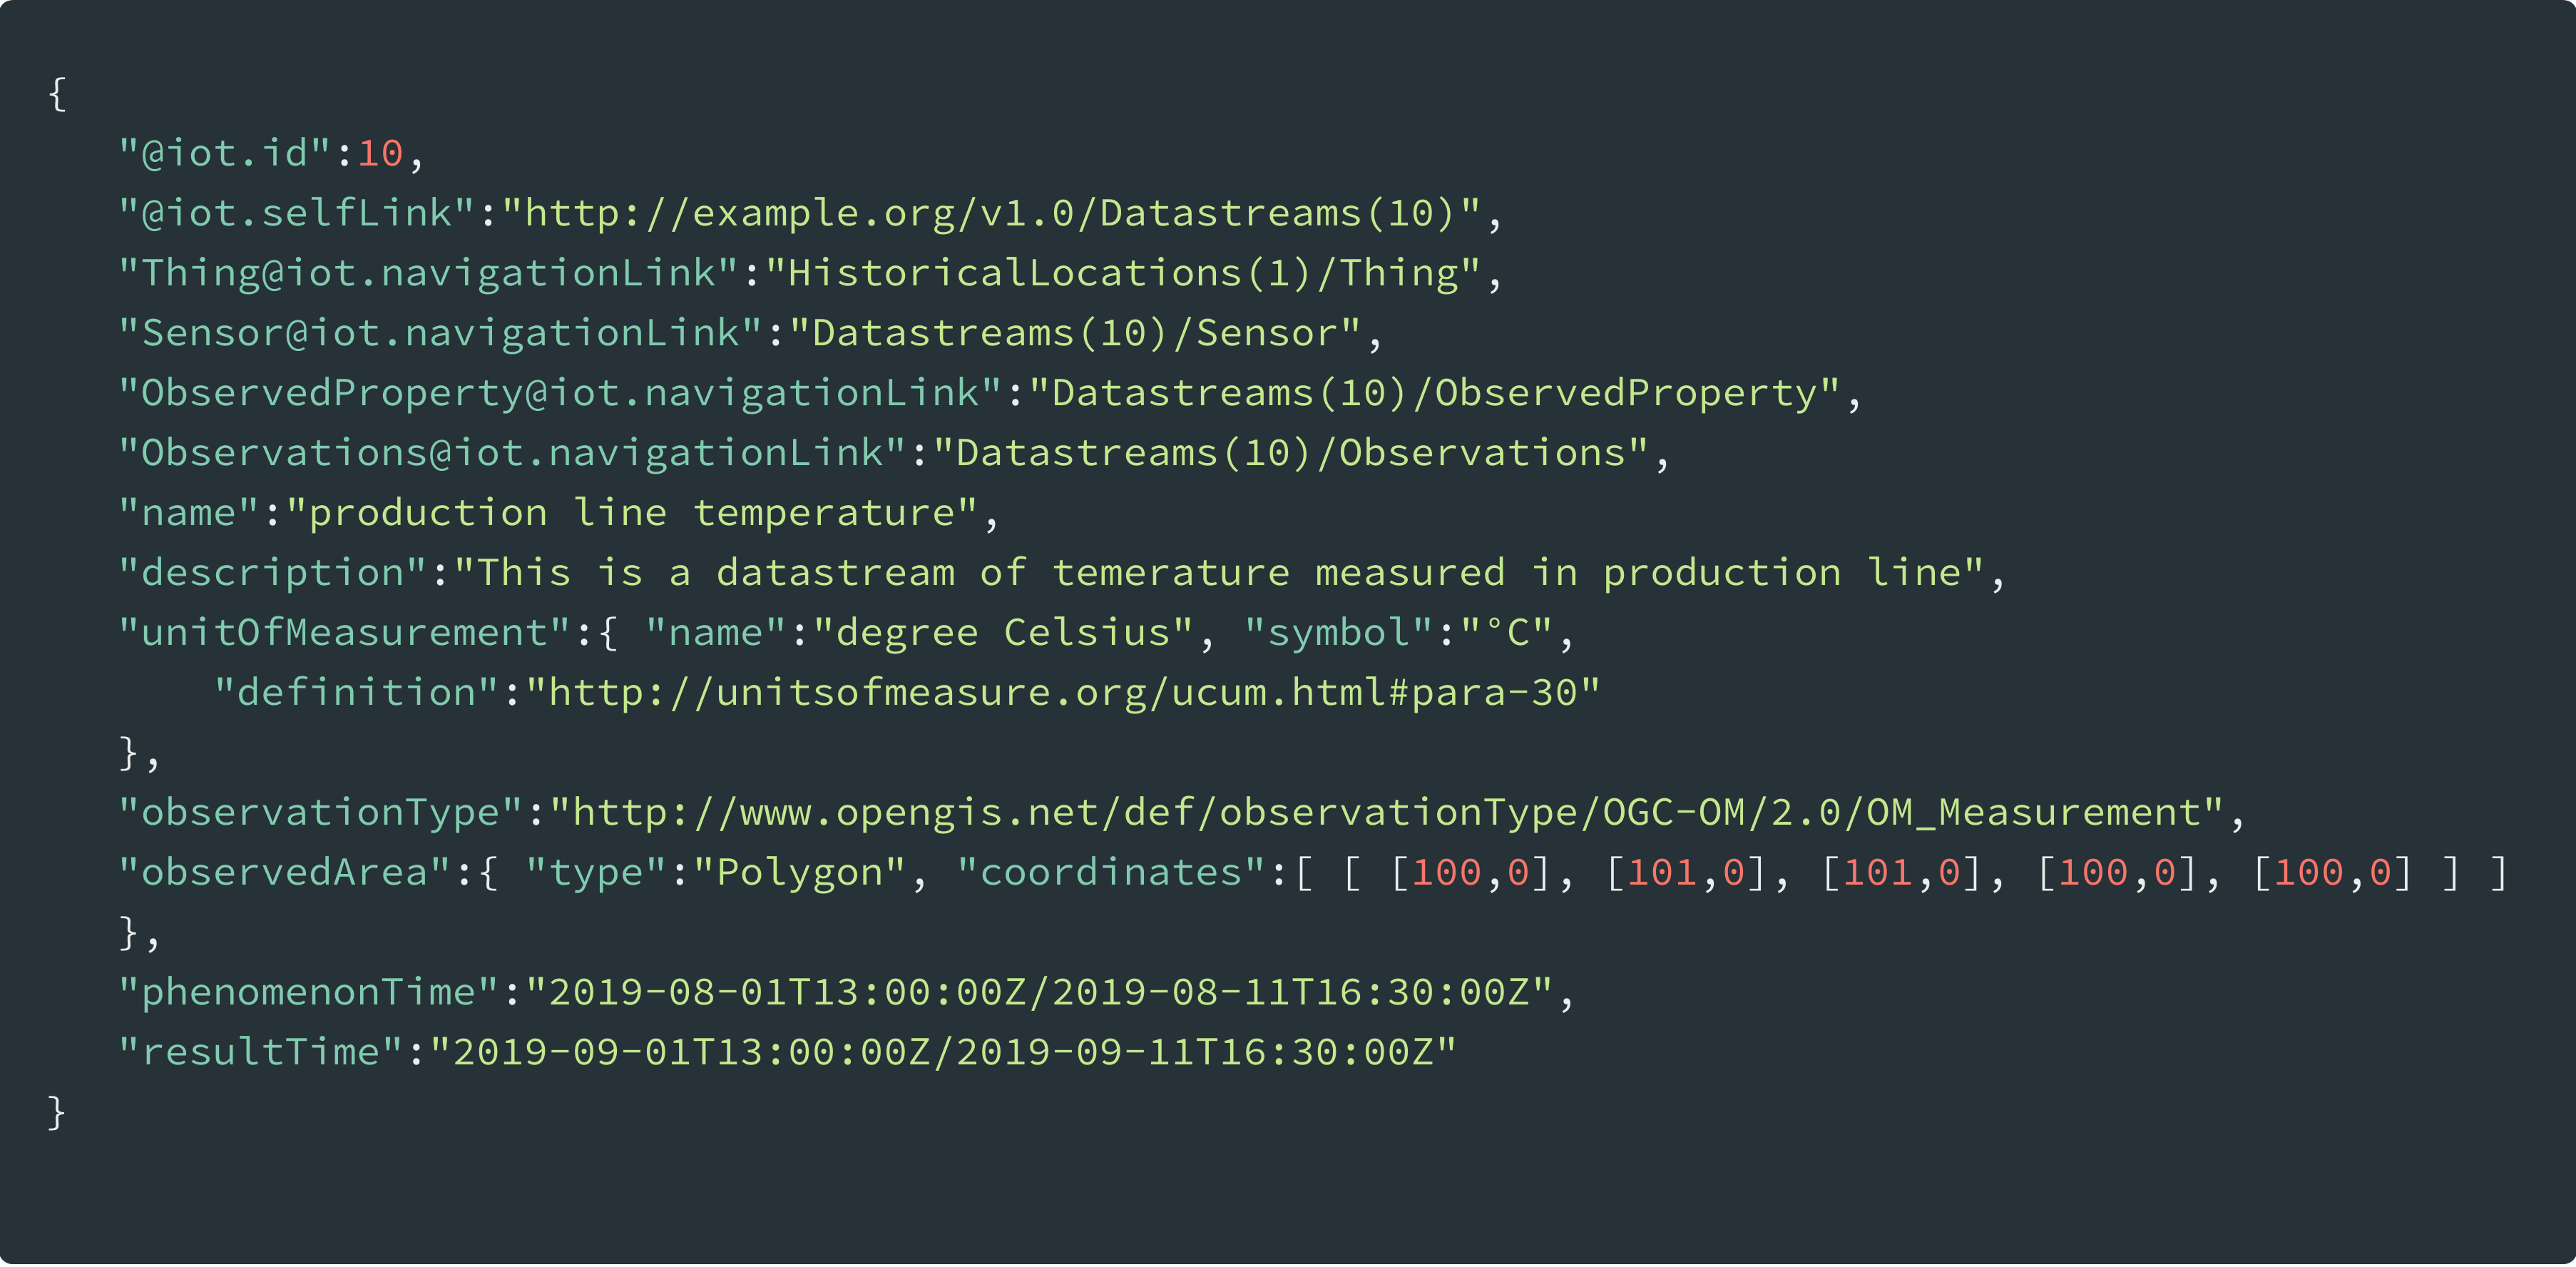
\includegraphics[scale=0.1]{./images/png/ogc/datastream}	
			\caption{Structure of Datastream entity}	
			\label{fig:datastream}	
		\end{center}
	\end{figure}


	\subsubsection{ObservedProperty}
	ObservedProperty shows what phenomenon is being observed by Observation entity. And it should have a data stream entity referenced to it.
	
	\begin{figure}[!htbp] 
		\begin{center}
			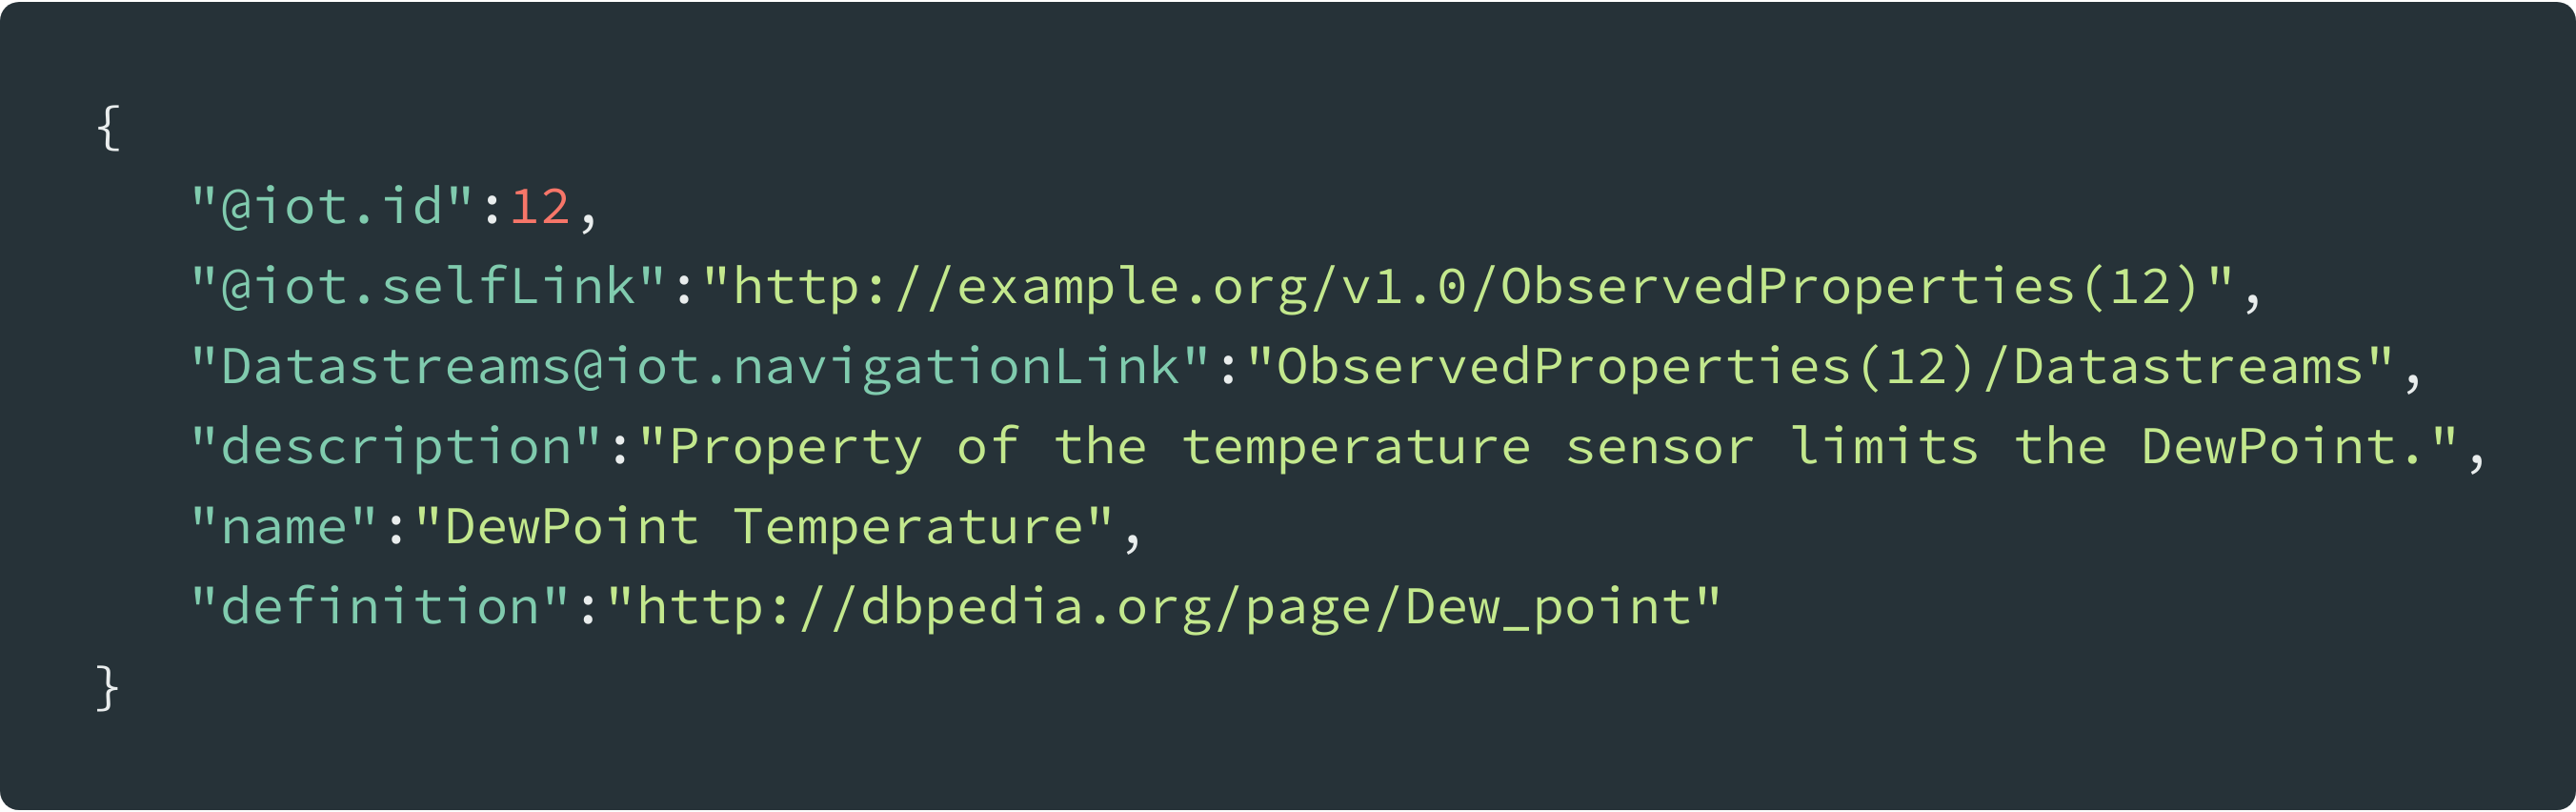
\includegraphics[scale=0.1]{./images/png/ogc/observedproperty}	
			\caption{Structure of ObservedProperty entity}	
			\label{fig:observedproperty}	
		\end{center}
	\end{figure}

	\subsubsection{Conclusion}
	OGC SensorThings API provide an open access to fetch all entities described above via HTTP network call, and it stores the data in a PostgreSQL relational database. Since their architecture supports only PostgreSQL we cannot use the complete component in our mediator. However, the standard given by OGC SensorThings makes a meaning relationship between entities in IoT systems. So, our proposed data model is designed based on the OGC SensorThings standards and it is explained in section \ref{subsubsection:schema_registry}. 

	\subsection{Resource Description Framework}

	Resource Description Framework (RDF) is a well known unique model to represent any resources in the universe with subject, predicate and object pattern like how humans communicate with each other.
	
	For example, consider a simple scenario where person one says to person two that "Christoper is a magician". In this statement 'Christoper' is subject, 'is a' is a predicate (relation) and 'magician' is an object. In a simple case, person two understands the statement if the person two knows only one Christoper in his/her life. However, if person two have a reference of multiple Christoper's, then it is unclear that which Christoper he/she is referring to? Then person two asks another question, which Christoper and where he is from? So now person one makes a new statement, "Christoper is from Bonn". In this statement, "Christopher" is the same subject, 'is from' a new predicate and "Bonn" is a new Object of type city. Now a person two enough information to infer which Christoper person one is talking about.
	
	\begin{figure}[!htbp] 
		\begin{center}
			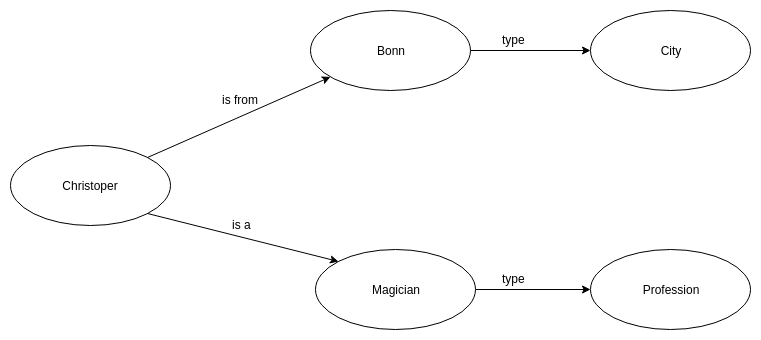
\includegraphics[scale=0.5]{./images/png/rdf/uml_example}	
			\caption{Illustrates a simple scenario in the form of RDF structure}	
			\label{fig:uml_example}	
		\end{center}
	\end{figure}

	Communication is way more easier between humans since they have a standard language model. However, What about machines? How can they communicate in a meaningful way? Alternatively, what if a person wants to communicate with a machine in the same way he/she communicates every day. This is where RDF plays a significant role in representing the data that a machine generates in a triples format aka Subject-Predicate-Object.
	
	\subsubsection{Components of RDF}
	
		RDF structure consists of two major components called Document and Statement. Document is the root container to have more than one RDF statements. In figure \ref{fig:rdf_document} 'xmlns:rdf' attribute represents the namespace of the current RDF document which gives a hint to the machines about how they can parse and understand this document.
		\begin{figure}[!htbp] 
			\begin{center}
				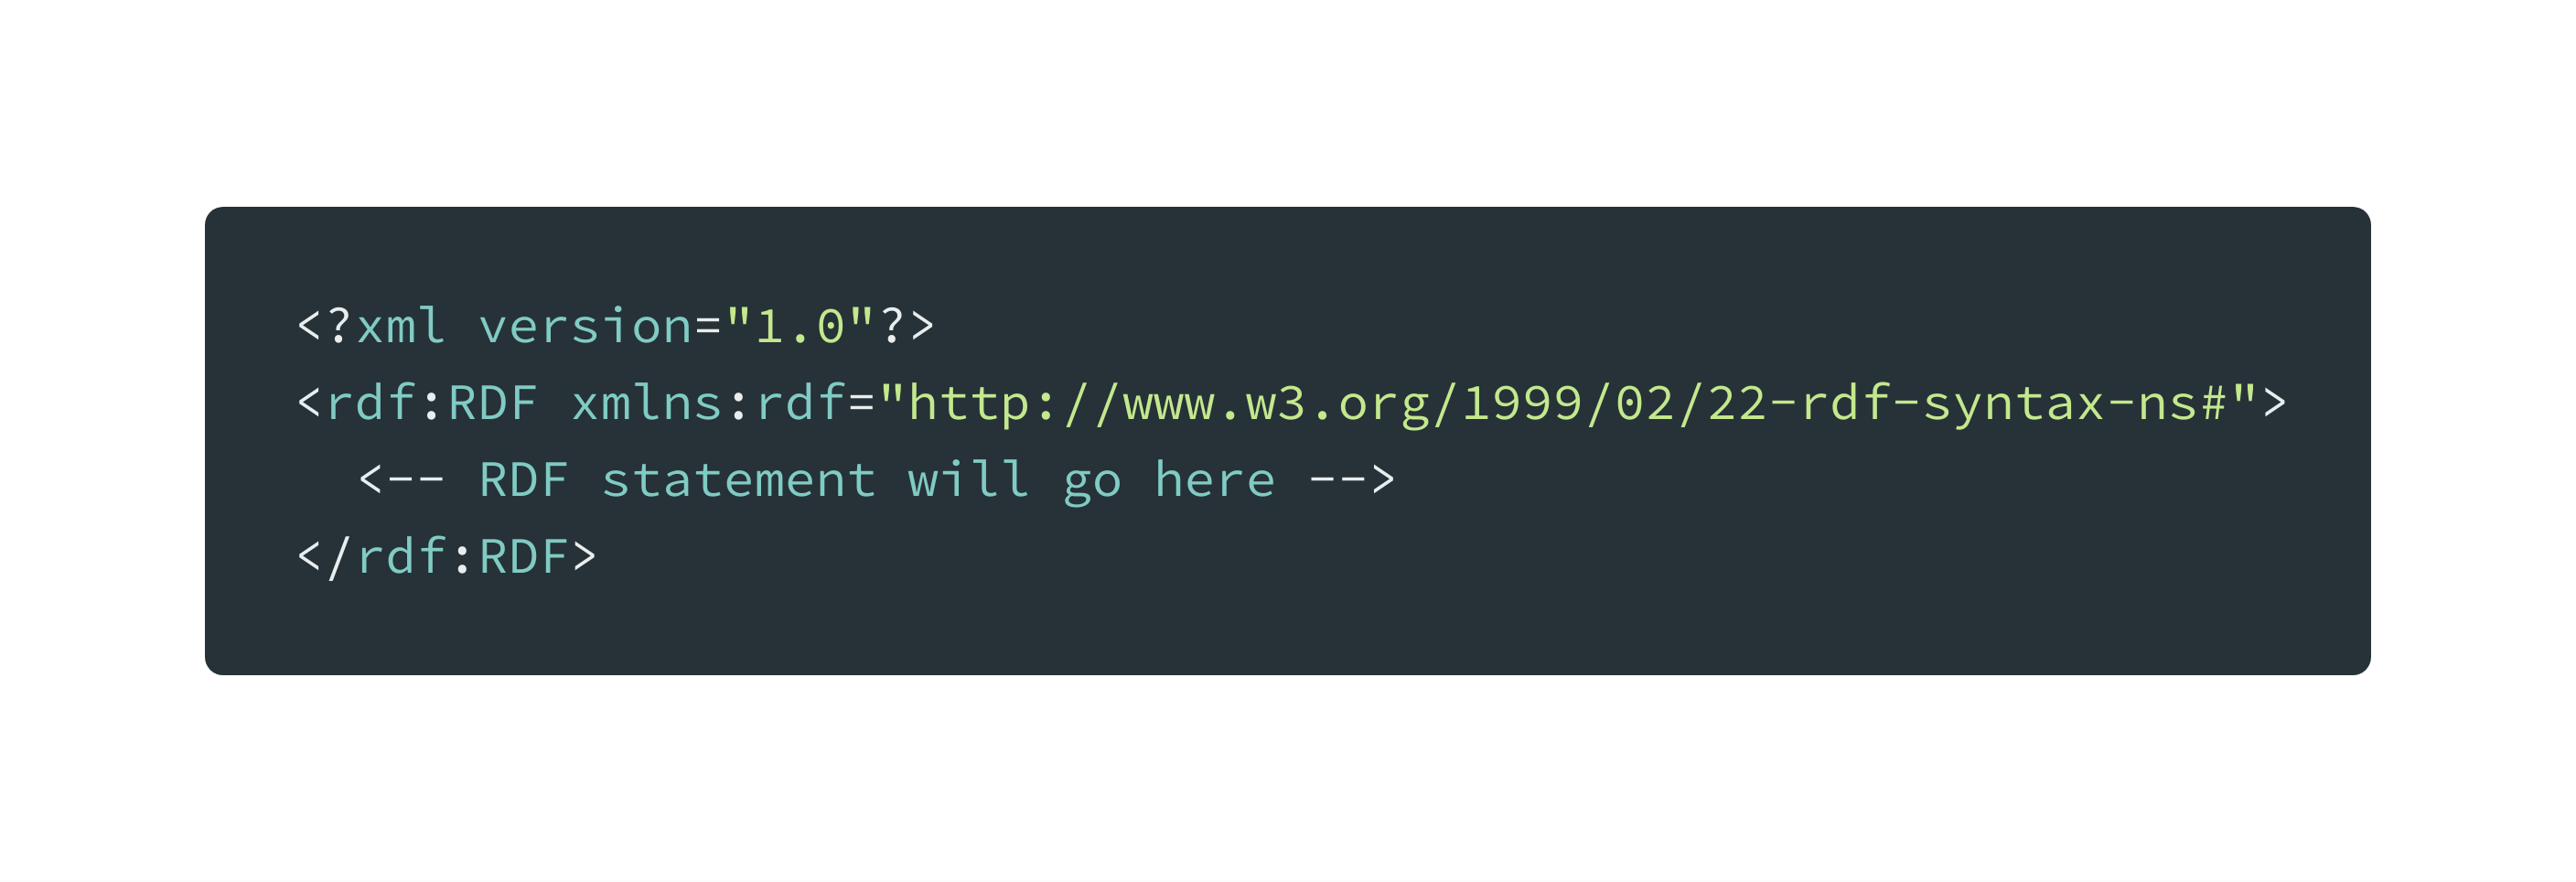
\includegraphics[scale=0.1]{./images/png/rdf/document}	
				\caption{Basic skeleton layout of Document}	
				\label{fig:rdf_document}	
			\end{center}
		\end{figure}
		
		Statement is a individual building block to represent a single triple. In the given example figure \ref{fig:rdf_statement}, RDF statement starts with subject description about Christoper and in the next level it have a predicate of 'is-a' pointing towards another resource 'Magician' which is an object in this statement. Each statement can have either a reference to other RDF statement or a value. 'Magician' and 'Bonn' statements in the example pointing to other RDF object via 'resource' attribute, and 'age' statement have a single value of '26' represents the age of the 'Christoper'.
		
		\begin{figure}[!htbp] 
			\begin{center}
				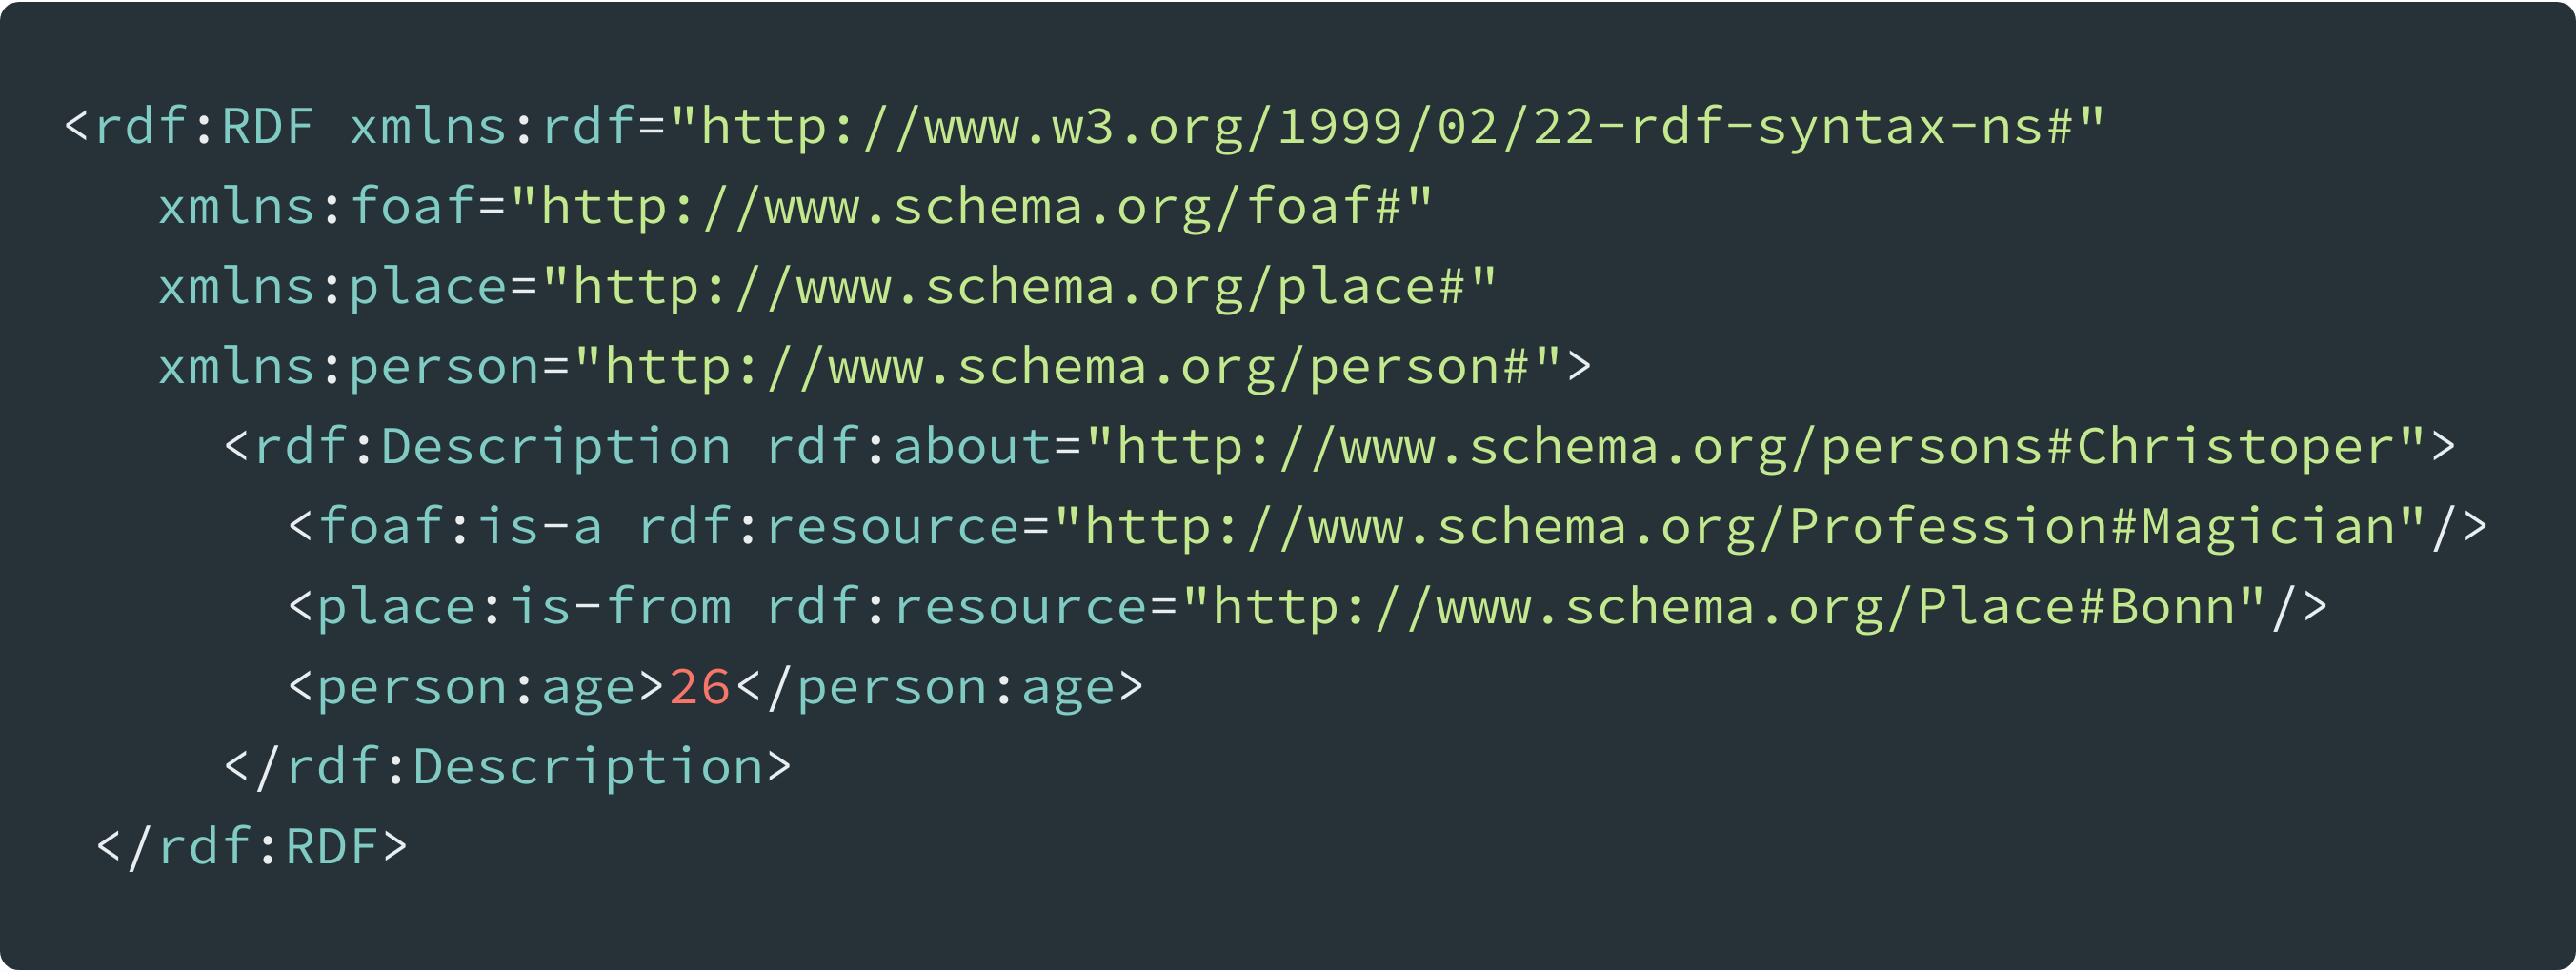
\includegraphics[scale=0.1]{./images/png/rdf/statement}	
				\caption{Basic skeleton layout of Statement}	
				\label{fig:rdf_statement}	
			\end{center}
		\end{figure}
	
		The primary advantage of adding semantics to the data is interoperability and easy to query them for a meaningful answer. Consider an example in the context of robotic applications. In multi-robot scenarios, more than one robot might work cooperatively to complete a single task. Let say, different vendors manufacture each robot, and the sensors generate values in different units or context. Robot one wants to share its current location information which is encoded by 'latitude and longitude' type to robot 2, and robot 2 sensor generates location information with 'geohash' encoding type. So whenever these robots share location values between them, it is not possible to consume it without the context of the values being encoded. If they share values along with encoding type as a context, then each robot can transform the values to the encoding type which is currently being used for the calculation.
		
		\subsection{JSON-LD}
		
		
		JSON-LD is an approach to structure the linked data and adding semantic contexts to data in the form of IRI (Internationalized Resource Identifier). An IRI is a unique and globally accessible link via web like URI, and the format is jointly defined by World Wide Web Consortium and Internet Engineering Task Force \cite{misc07}. Let us try to understand how JSON-LD solves interoperability issues with a toy example. Consider we have two robots developed by different developers and each publishing ROS Twist messages at a specific rate.
		
		Developers of the first robot decided to publish the twist messages with the following format.
		
		\begin{figure}[!htbp] 
			\begin{center}
				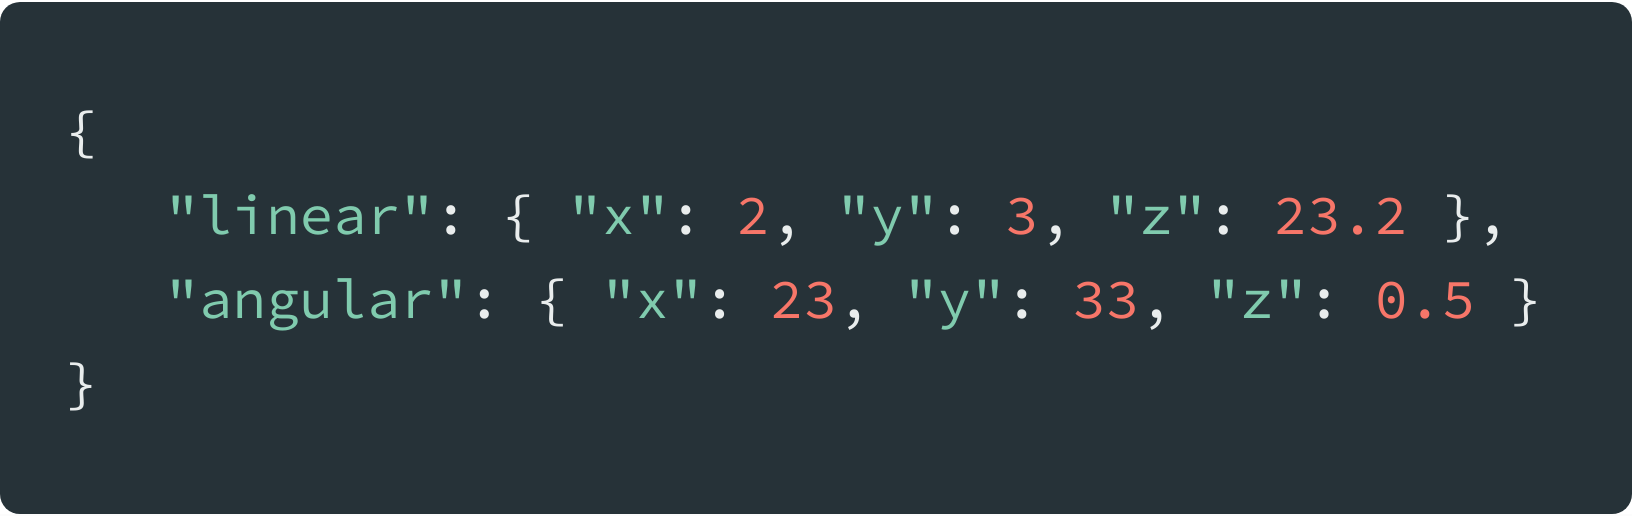
\includegraphics[scale=0.1]{./images/png/jsonld/1}	
				\caption{Twist message created by robot one}	
				\label{fig:jsonld_1}	
			\end{center}
		\end{figure}
	
		Developers of the second robot decided to publish the twist messages with the following format.
	
		\begin{figure}[!htbp] 
			\begin{center}
				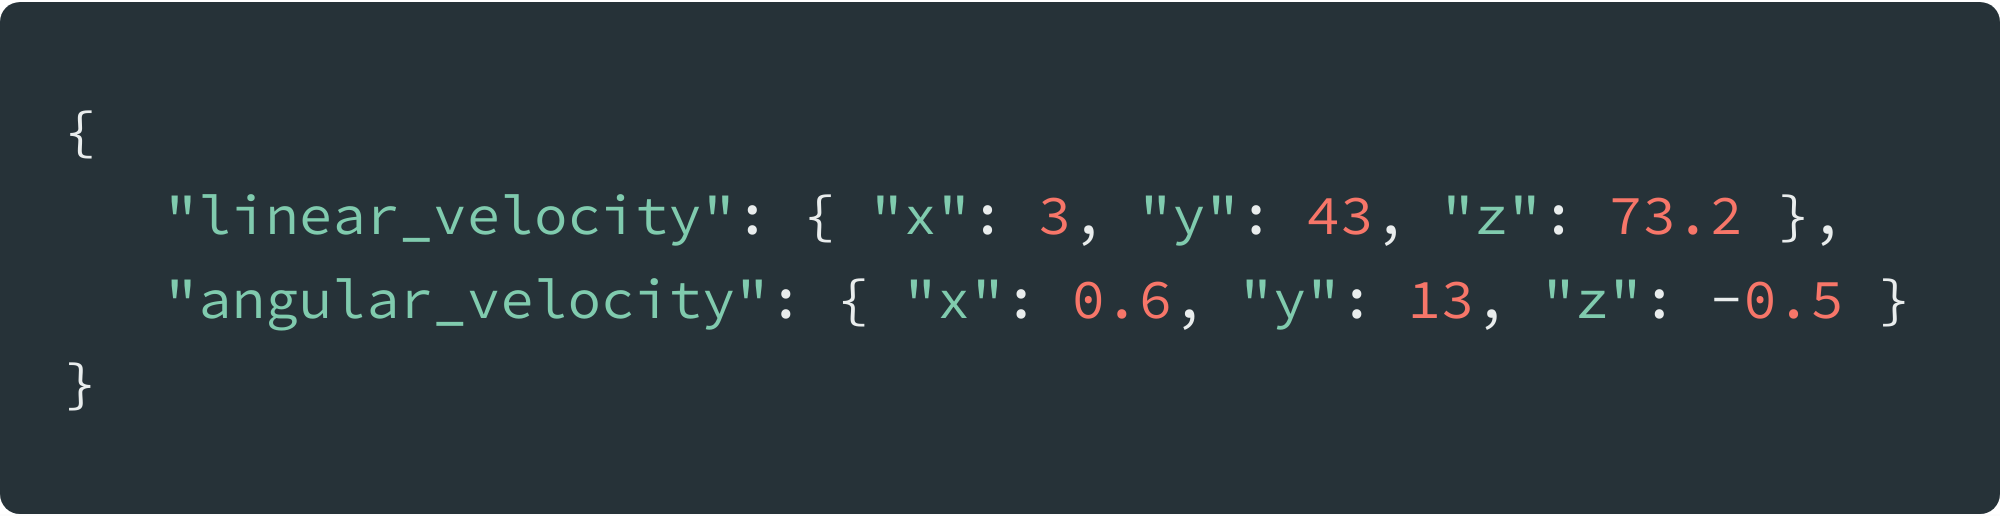
\includegraphics[scale=0.1]{./images/png/jsonld/2}	
				\caption{Twist message created by robot two}	
				\label{fig:jsonld_2}	
			\end{center}
		\end{figure}
	
		We can see from both the format, underlying data is the same, but the representation is different. In the first robot, the linear and angular velocity has been identified with the keys "linear" and "angular", and in the second robot, the same data will be identified with the keys "linear\_velocity" and "angular\_velocity". In a multi-robot environment, if all the robots know what data they are exchanging and how it has been encoded, then there are no issues. However, what if two stranger robots want to communicate or transfer data with each other? For example, robot one wants to navigate from one location to another without colliding with other robots in the environment. With the formats mentioned above, robot one cannot understand what robot two is saying, because they do not talk in the same language.
		
		This is where JSON-LD plays a significant role to solve this interoperability issue. Let solve the issue discussed above with the help of JSON-LD.
		
		\begin{figure}[!htbp] 
			\begin{center}
				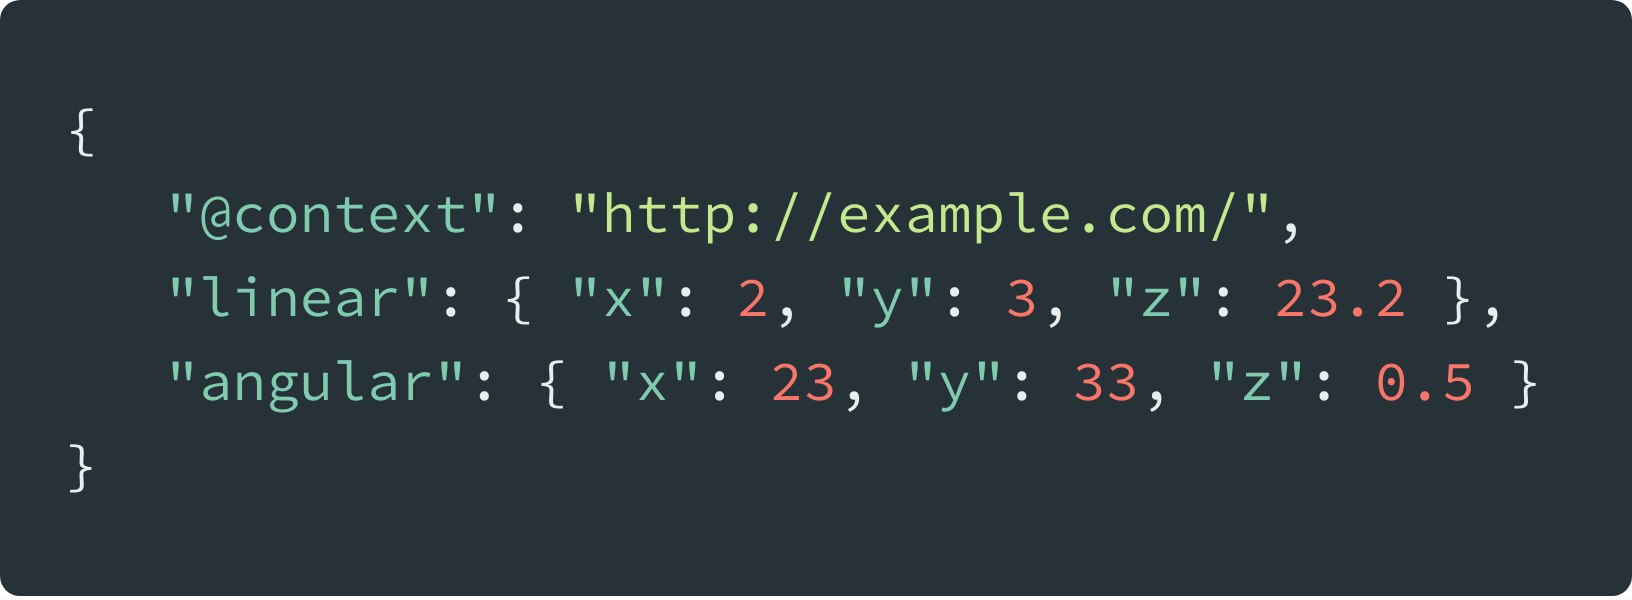
\includegraphics[scale=0.1]{./images/png/jsonld/3}	
				\caption{Twist message created by robot one in JSON-LD format}	
				\label{fig:jsonld_3}	
			\end{center}
		\end{figure}
	
		What has been changed in the first robot twist message? We have added a "@context" keyword to the existing message. This means that, whoever consumes this message, they have to understand the complete message in the context of "http://example.com/". Now we transform the second robot message format like this.
		
		\begin{figure}[!htbp] 
			\begin{center}
				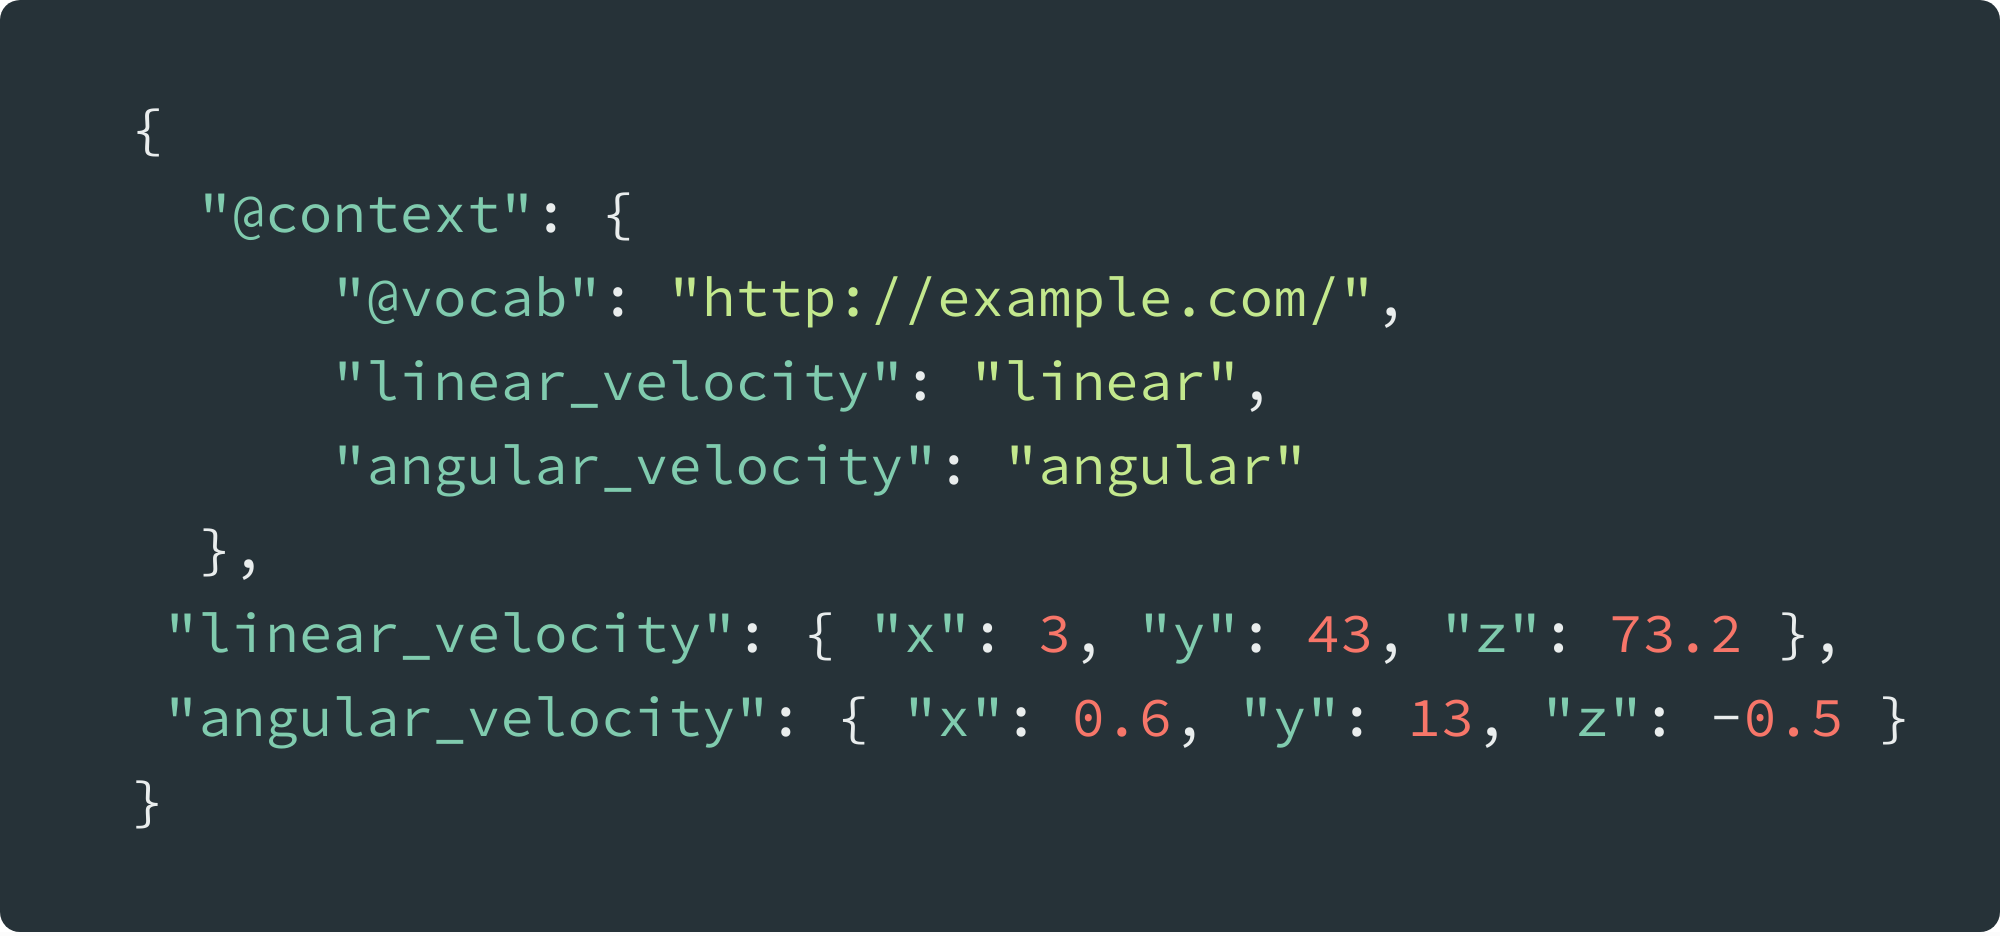
\includegraphics[scale=0.1]{./images/png/jsonld/4}	
				\caption{Transformed twist message created by robot two in JSON-LD format}	
				\label{fig:jsonld_4}	
			\end{center}
		\end{figure}	
	
		In the new transformation, we added one more attribute called "@vocab" which means that apply the "http://example.com/" IRI to all keys with the specific key mapping. Now one may think that how this solves the interoperability issue? Still, both messages look exactly different with few extra @context and @vocab information.
		
		JSON-LD does not offer only the semantic representation, but also offers two other important features called Expansion and Compaction algorithm.
		
	\subsubsection{Expansion algorithm}
		
	Expansion algorithm takes an object as an input along with its context and applies the context into the data attributes and expands all compact IRIs to absolute IRIs. Also, during the expansion, it expresses all JSON-LD values in the expanded form. Finally, it removes the "@context" information from the result data since all information is propagated to the real data. Let us apply the expansion algorithm on the twist messages created by robot one and two, and see the result after applying the expansion algorithm.

	
		\begin{figure*}[!htbp]
		\subfloat[Transformed twist message created by robot one after applying expansion algorithm\label{subfig-1:jsonld_5}]{%
			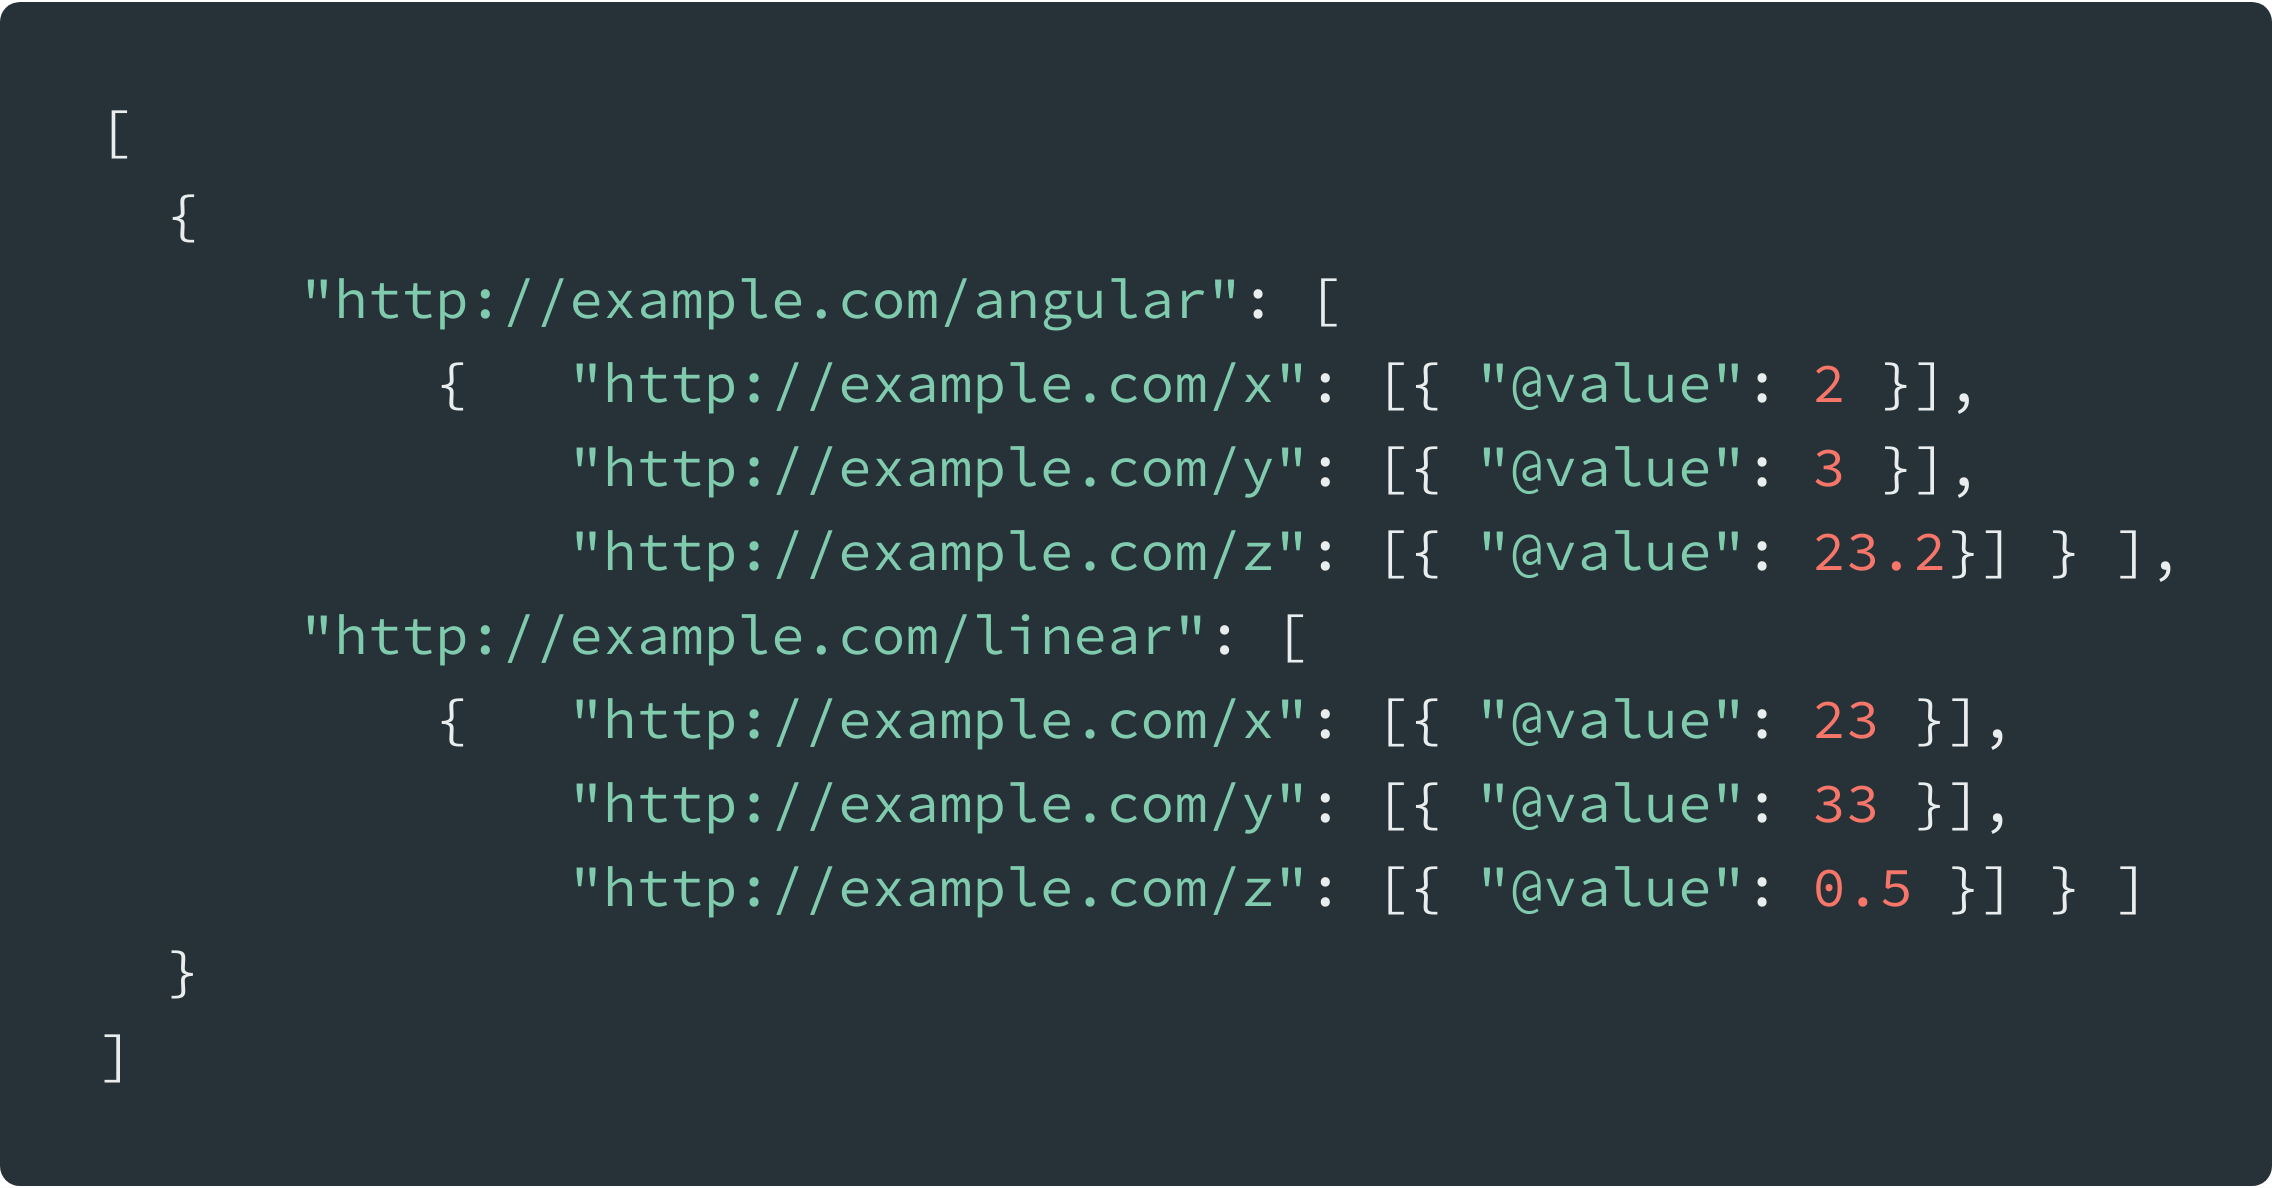
\includegraphics[scale=0.1]{./images/png/jsonld/5}
		}
		\hfill
		\subfloat[Transformed twist message created by robot two after applying expansion algorithm\label{subfig-2:jsonld_6}]{%
			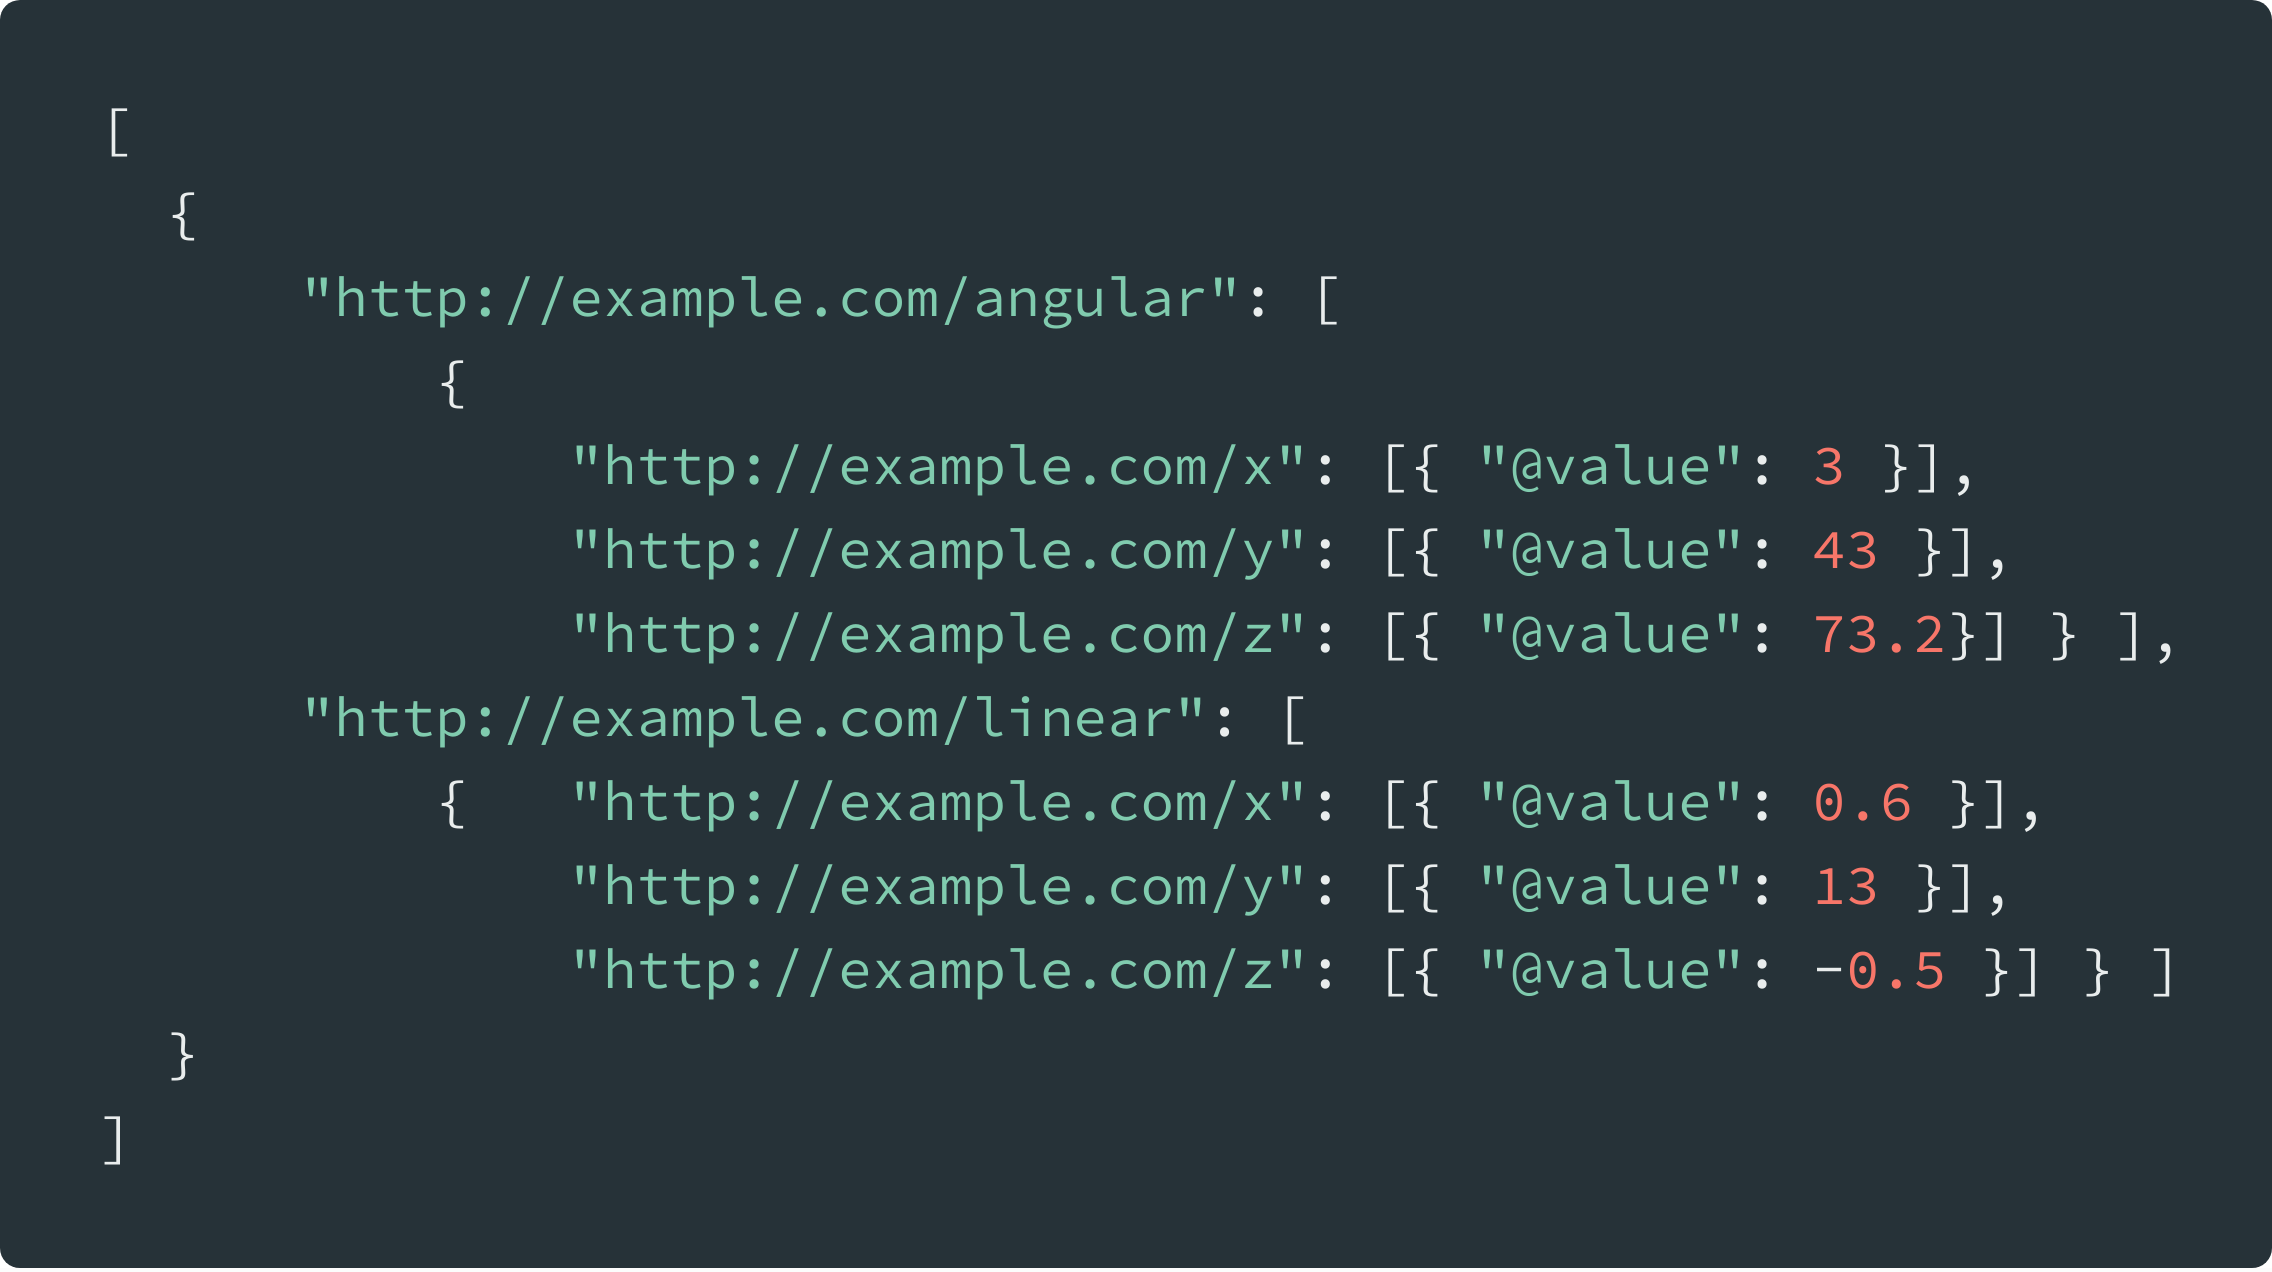
\includegraphics[scale=0.094]{./images/png/jsonld/6}
		}
		\caption{Twist messages from robot one and two}
		\label{fig:dummy}
	\end{figure*}
	Now both the messages in figure \ref{subfig-1:jsonld_5}, \ref{subfig-2:jsonld_6} look exactly the same without any difference in keys. This is the power of JSON-LD expansion algorithm. One can probably think now, who creates the common vocabulary list which can be understandable by all the robots. So far, there are many vocabulary lists has been created for common things in the universe but ain't one for robots ecosystem. For example,
	
	
	\begin{itemize}
		\item https://schema.org/ - schema.org have a vast collection of most common definable things in the universe.
		\item http://thingschema.org/ - thingsschema.org has just initiated a motivation to define things (smart things) in the environment.
		\item https://iot.schema.org/ - iot.schema.org defines the vocabulary list and relationships for IoT devices.
		\item https://wiki.dbpedia.org/ - dbpedia.org have a collection of person record to identify each person information in the world uniquely.
	\end{itemize}

	As part of this research work, we are taking the initiative to prepare a set of vocabs for robots, sensors and its working environment. Then, we use the vocabularies to represent robot generated messages with more precise context so that any other robots in the world can understand each other even though different vendors are manufacturing them.
	
	\subsubsection{Compaction algorithm}
	
	Compaction algorithm takes two inputs, one is the real data object \ref{fig:jsonld_compaction_1} and the second is an object \ref{fig:jsonld_compaction_2} which has only context information and generates a human-readable final result \ref{fig:jsonld_compaction_3} which includes both data and context injected into it.
	
			\begin{figure}[!htbp] 
		\begin{center}
			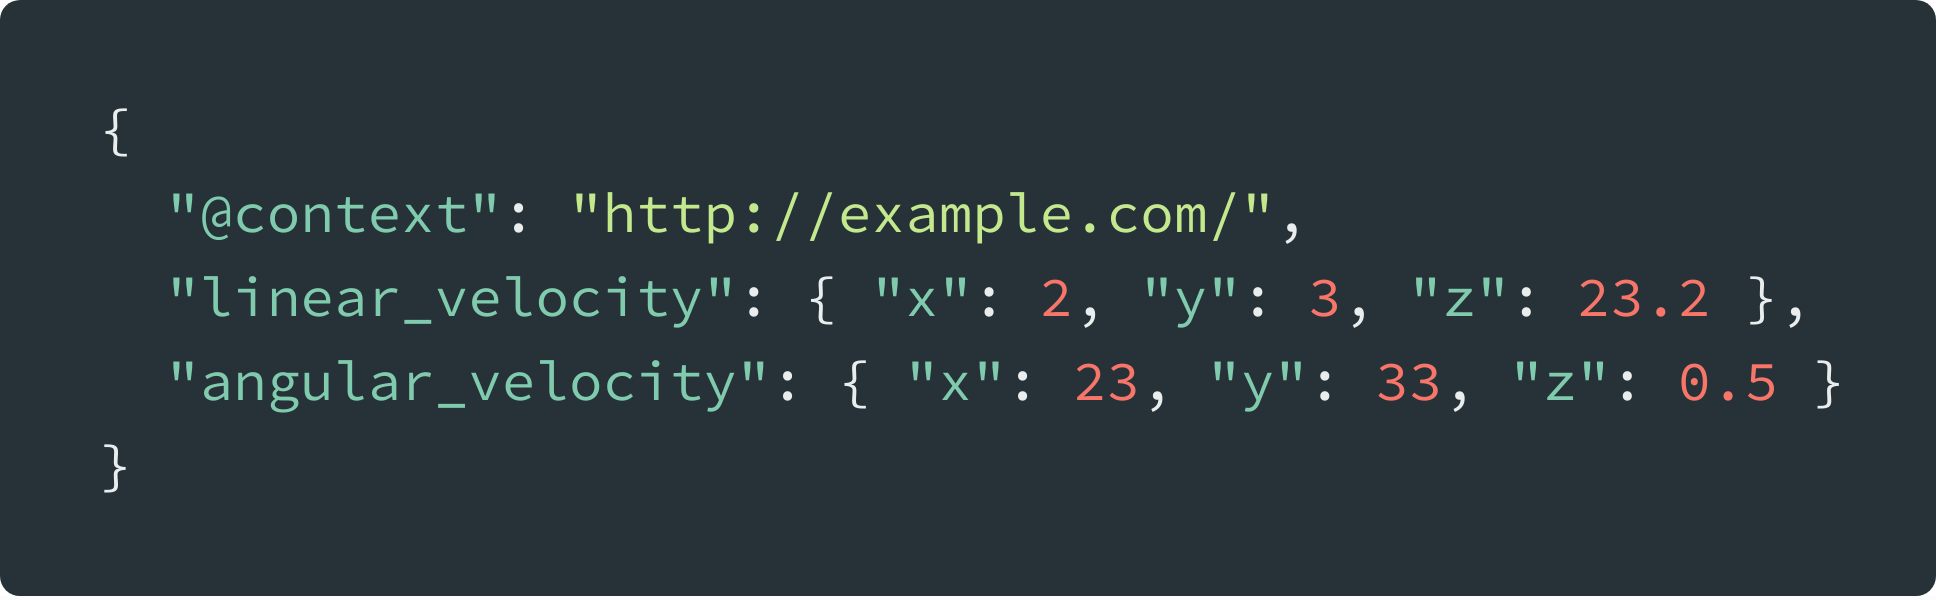
\includegraphics[scale=0.1]{./images/png/jsonld/compaction_1}	
			\caption{First input to the compaction algorithm}	
			\label{fig:jsonld_compaction_1}	
		\end{center}
	\end{figure}
	
	\begin{figure}[!htbp] 
		\begin{center}
			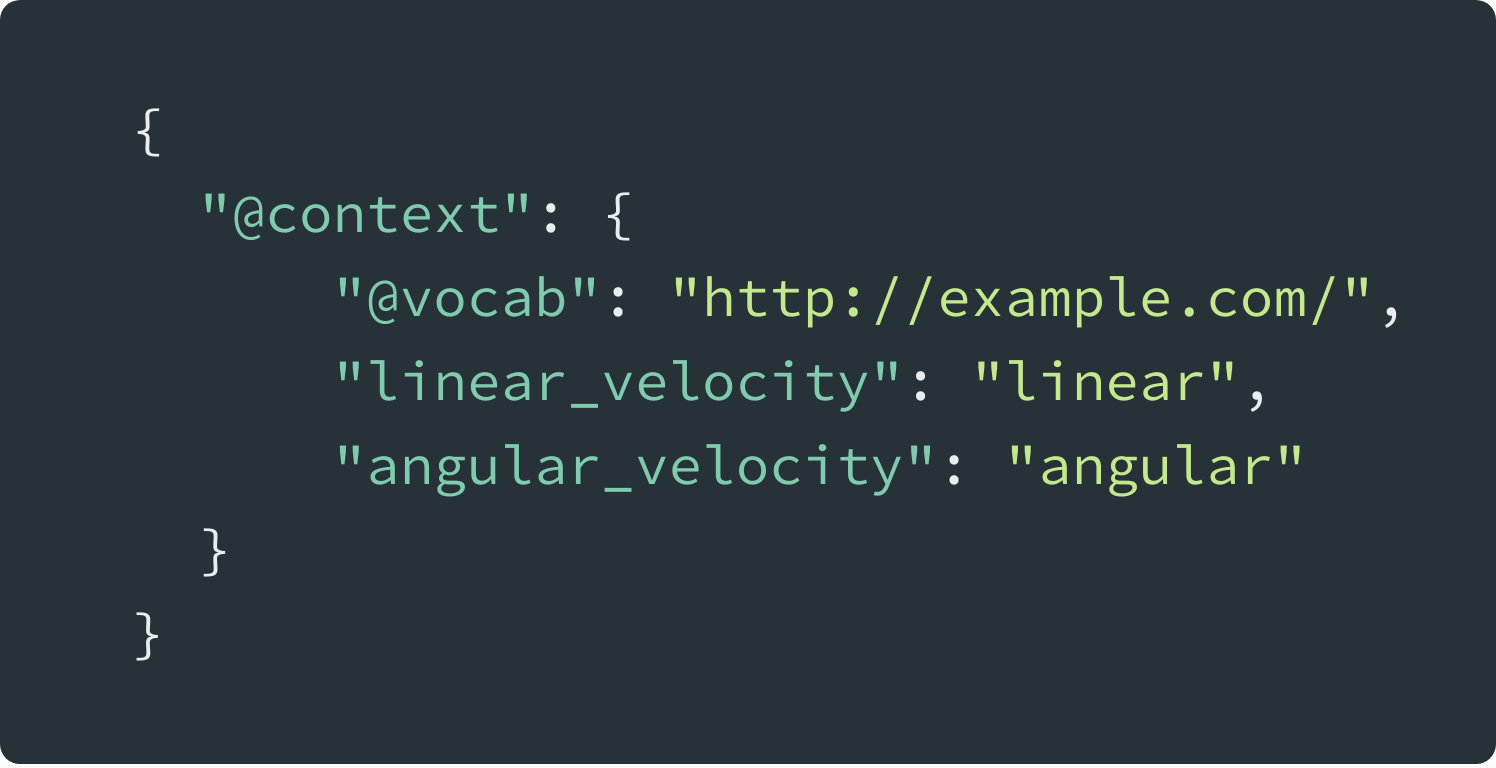
\includegraphics[scale=0.1]{./images/png/jsonld/compaction_2}	
			\caption{Second input to the compaction algorithm}	
			\label{fig:jsonld_compaction_2}	
		\end{center}
	\end{figure}
	

	\begin{figure}[!htbp] 
		\begin{center}
			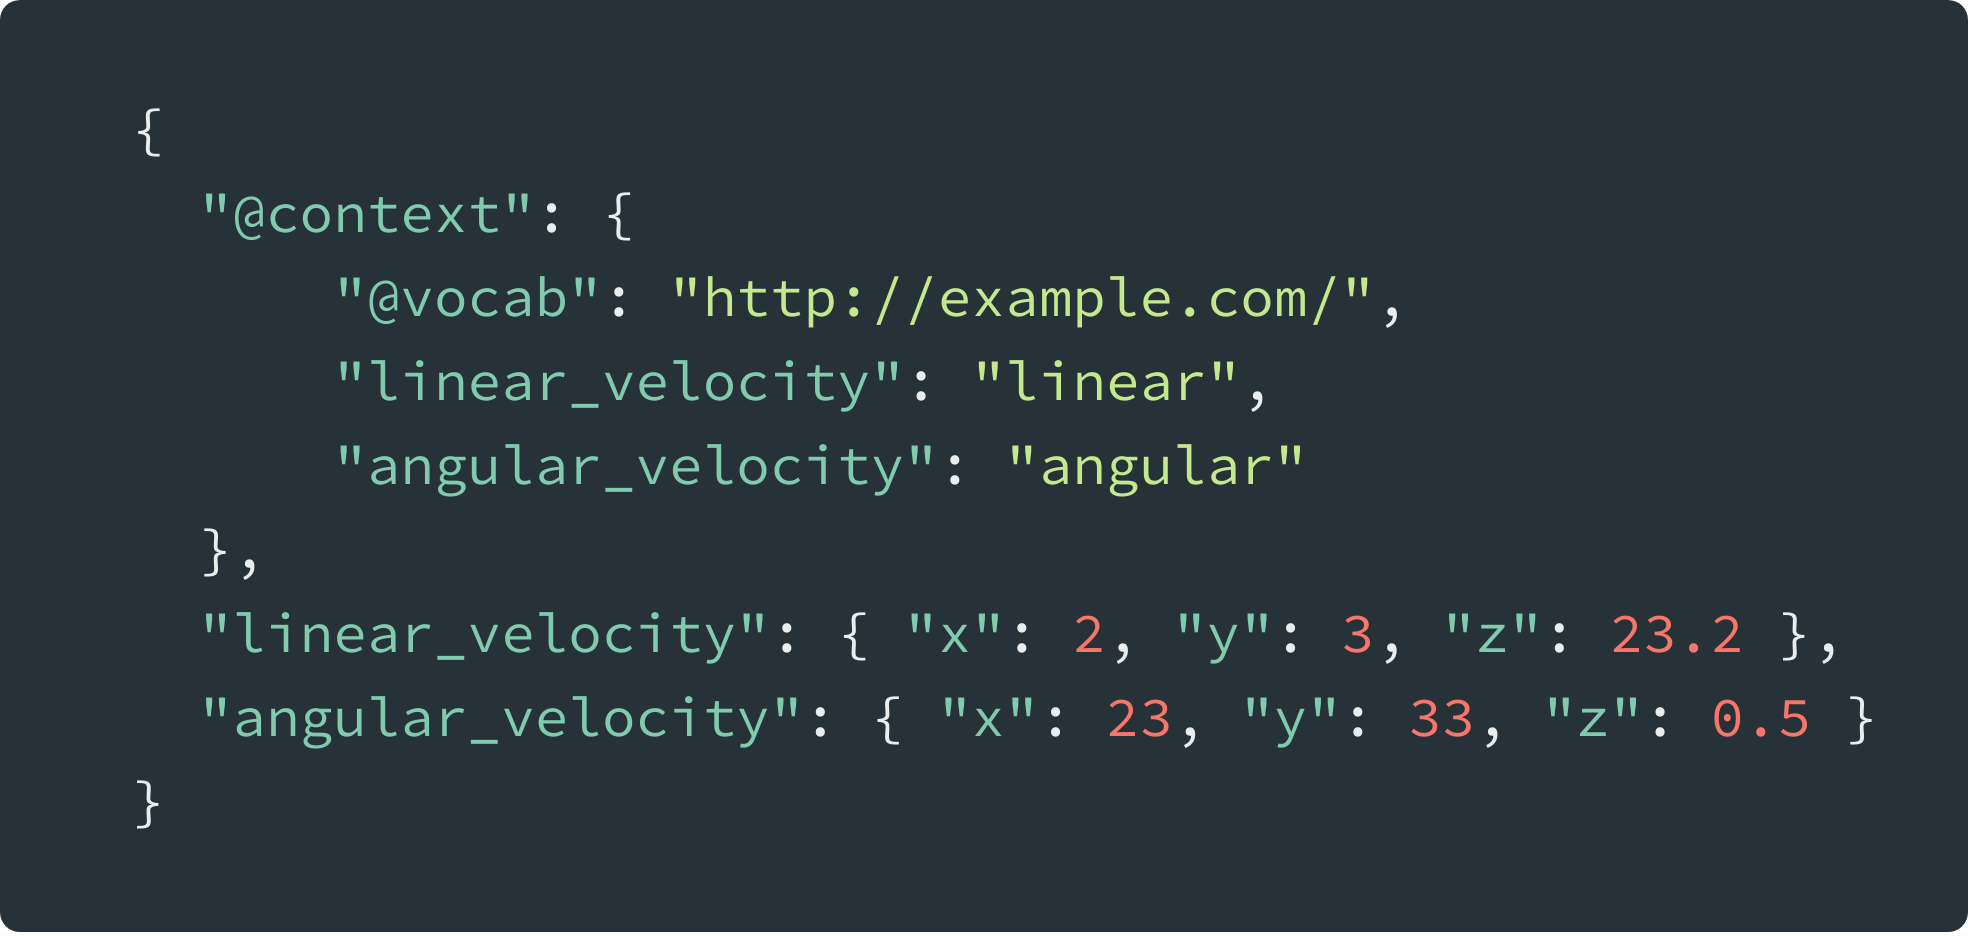
\includegraphics[scale=0.1]{./images/png/jsonld/compaction_3}	
			\caption{Result produced by compaction algorithm}	
			\label{fig:jsonld_compaction_3}	
		\end{center}
	\end{figure}	

	As it is stated above, "@context" is injected into the real data object. Now the result object can contextually understandable by other robots.
		
		
		\subsubsection{Why JSON -LD instead of JSON?}
		
		JSON is a widely used format to exchange data between systems and storing persistently in databases. Also, there are many famous document based databases(e.g., MongoDB, CouchDB, etc.) evolved which supports handling JSON objects. Any system can easily parse JSON objects, but the JSON object itself is meaningless. The context of each key can be shared manually with any form of documentation, but it is not easily accessible every time.
		
		For example, a developer worked on a system and named the keys by his own interest. Now if a new developer wants to understand what a specific key means, then he/she needs to check the document or contact other developers. It is even more difficult for machines, to interpret what each key means in a JSON object. JSON-LD solves this problem by encoding IRI's in the JSON object to uniquely identify each key.
		
		
	
\end{document}
